% Options for packages loaded elsewhere
\PassOptionsToPackage{unicode}{hyperref}
\PassOptionsToPackage{hyphens}{url}
\PassOptionsToPackage{dvipsnames,svgnames,x11names}{xcolor}
\documentclass[
  11pt,
]{article}
\usepackage{xcolor}
\usepackage[margin=1in]{geometry}
\usepackage{amsmath,amssymb}
\setcounter{secnumdepth}{5}
\usepackage{iftex}
\ifPDFTeX
  \usepackage[T1]{fontenc}
  \usepackage[utf8]{inputenc}
  \usepackage{textcomp} % provide euro and other symbols
\else % if luatex or xetex
  \usepackage{unicode-math} % this also loads fontspec
  \defaultfontfeatures{Scale=MatchLowercase}
  \defaultfontfeatures[\rmfamily]{Ligatures=TeX,Scale=1}
\fi
\usepackage{lmodern}
\ifPDFTeX\else
  % xetex/luatex font selection
\fi
% Use upquote if available, for straight quotes in verbatim environments
\IfFileExists{upquote.sty}{\usepackage{upquote}}{}
\IfFileExists{microtype.sty}{% use microtype if available
  \usepackage[]{microtype}
  \UseMicrotypeSet[protrusion]{basicmath} % disable protrusion for tt fonts
}{}
\makeatletter
\@ifundefined{KOMAClassName}{% if non-KOMA class
  \IfFileExists{parskip.sty}{%
    \usepackage{parskip}
  }{% else
    \setlength{\parindent}{0pt}
    \setlength{\parskip}{6pt plus 2pt minus 1pt}}
}{% if KOMA class
  \KOMAoptions{parskip=half}}
\makeatother
\usepackage{longtable,booktabs,array}
\usepackage{caption}
\captionsetup[table]{skip=6pt}
\newcounter{none} % for unnumbered tables
\usepackage{calc} % for calculating minipage widths
% Correct order of tables after \paragraph or \subparagraph
\usepackage{etoolbox}
\makeatletter
\patchcmd\longtable{\par}{\if@noskipsec\mbox{}\fi\par}{}{}
\makeatother
\setlength{\emergencystretch}{3em} % prevent overfull lines
\providecommand{\tightlist}{%
  \setlength{\itemsep}{0pt}\setlength{\parskip}{0pt}}
\usepackage{microtype}
\usepackage{fancyhdr}
\usepackage{longtable,booktabs}
\usepackage{tikz}
\usetikzlibrary{arrows.meta,positioning,calc}
\definecolor{NimbusBlue}{HTML}{233F58}
\definecolor{NimbusLight}{HTML}{EDF3F7}
\AtBeginDocument{\hypersetup{linkcolor=NimbusBlue,filecolor=NimbusBlue,urlcolor=NimbusBlue,citecolor=NimbusBlue}}
\setlength{\emergencystretch}{3em}
\setlength{\parskip}{0.45em}
\setlength{\parindent}{0pt}
\pagestyle{fancy}
\fancyhf{}
\fancyhead[L]{\small\sffamily Nimbus}
\fancyhead[R]{\small\sffamily Technical documentation}
\fancyfoot[C]{\small\thepage}
\renewcommand{\headrulewidth}{0.3pt}
\AtBeginDocument{\setlength{\headheight}{15pt}}
\providecommand{\tightlist}{\setlength{\itemsep}{0pt}\setlength{\parskip}{0pt}}

\usepackage{bookmark}
\IfFileExists{xurl.sty}{\usepackage{xurl}}{} % add URL line breaks if available
\urlstyle{same}
% fallback for those not using the hyperref driver hyperxmp:
\makeatletter
\@ifundefined{xmpquote}{\newcommand{\xmpquote}[1]{#1}}{}
\makeatother
\hypersetup{
  pdftitle={Nimbus: Architecture and design choices},
  pdfauthor={Nimbus project documentation},
  colorlinks=true,
  linkcolor={Maroon},
  filecolor={Maroon},
  citecolor={Blue},
  urlcolor={Blue},
  pdfcreator={LaTeX via Tectonic}}

\title{Nimbus: Architecture and design choices}
\author{Nimbus project documentation}
\date{18 October 2026}

\begin{document}
\hypersetup{pageanchor=false}
\maketitle
\hypersetup{pageanchor=true}
\pagenumbering{roman}

{
\small
\setlength{\parskip}{0pt}
\setcounter{tocdepth}{2}
\tableofcontents
}
\clearpage
\pagenumbering{arabic}
\pagestyle{fancy}
Nimbus separates the atmospheric calculation from the application used
to configure and inspect it. The simulator is a C++17 executable, independently
developed rather than ported or forked from CM1. Nimbus Studio is a Tauri
desktop application: TypeScript and React provide the
interface, while Rust owns filesystem access, process control and native
data readers. Studio launches the simulator as a separate process. The
same executable can run from a terminal or on a remote Linux computer
without an open Studio window.

This boundary makes a saved configuration and the simulator that
interpreted it the starting point for reproducibility. A plot is a view
of a completed simulation product, rather than part of the atmospheric
time integration. The \href{MATHEMATICS.pdf}{mathematics guide} explains the
physical and numerical assumptions; this guide explains where those
assumptions are enforced and who owns the data. The execution chapters follow
configuration, host storage, CPU portability, GPU submission and numerical
precision. The publication chapters then trace persistence and IPC; the
rendering chapter follows those published values through shaders to pixels.
The final chapters separate performance models, historical observations and
the evidence required for a new change.

\begin{figure}[htbp]
\centering
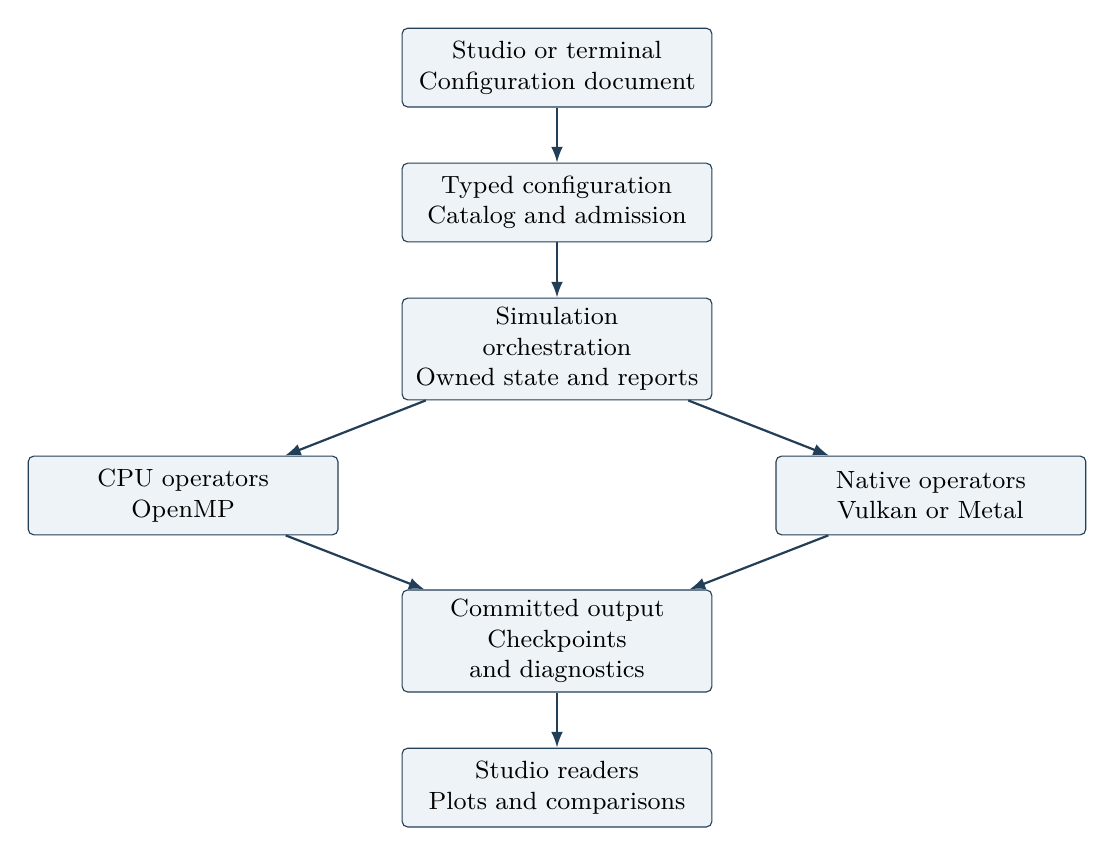
\begin{tikzpicture}[
  box/.style={draw=NimbusBlue,fill=NimbusLight,rounded corners=2pt,
              text width=3.7cm,minimum height=1cm,align=center,font=\small},
  arrow/.style={-{Latex[length=2mm]},draw=NimbusBlue,thick},
  node distance=7mm and 8mm]
  \node[box] (input) {Studio or terminal\\Configuration document};
  \node[box,below=of input] (admission) {Typed configuration\\Catalog and admission};
  \node[box,below=of admission] (orchestration) {Simulation\\orchestration\\Owned state and reports};
  \node[box,below left=of orchestration] (cpu) {CPU operators\\OpenMP};
  \node[box,below right=of orchestration] (gpu) {Native operators\\Vulkan or Metal};
  \node[box,below=24mm of orchestration] (output) {Committed output\\Checkpoints and diagnostics};
  \node[box,below=of output] (view) {Studio readers\\Plots and comparisons};
  \draw[arrow] (input)--(admission);
  \draw[arrow] (admission)--(orchestration);
  \draw[arrow] (orchestration)--(cpu);
  \draw[arrow] (orchestration)--(gpu);
  \draw[arrow] (cpu)--(output);
  \draw[arrow] (gpu)--(output);
  \draw[arrow] (output)--(view);
\end{tikzpicture}
\caption{The application and solver share configuration and publication contracts.
The numerical state remains owned by the solver. Backend-specific memory and
synchronization operate inside that ownership boundary.}
\end{figure}


\section{Local experimentation and the decision to use HPC}
\label{architecture-local-experiments}

A central goal is high-fidelity atmospheric simulation on ordinary workstations
and MacBooks through efficient algorithms, careful memory ownership and GPU
acceleration. Local work is not intended to stop at toy models, coarse previews
or preliminary checks before an inevitable cluster run. Reducing avoidable
work and data movement can make substantially more demanding experiments
practical on the same hardware. A researcher
should be able to change a documented experiment, inspect its assumptions,
and increase its resolution without maintaining a separate solver fork for
each case. The objective is useful scientific work per unit of time, memory
and effort. A high GPU utilization percentage is not sufficient evidence of
that objective, and a run does not become scientifically adequate merely
because it completes on a laptop or a cluster.

Three questions determine where an experiment belongs. First, does the
discretization and selected physics answer the scientific question? Second,
does the complete working set fit the available resources? Third, can the
required duration, repetitions and analysis finish within the researcher's
time budget? A configuration can pass one question and fail another. The
\href{MATHEMATICS.pdf}{mathematics guide's resolution and experiment-design
chapter} develops the first question and the scaling assumptions behind the
other two. This section describes the engineering boundaries that keep the
answers separate.

\subsection{Capacity and turnaround are different constraints}

A useful memory estimate follows simultaneously live owners. It includes
primary fields, time-integration stages, scheme-private state, geometry,
rollback candidates, reports, output snapshots and communication buffers.
The simulator, Studio, Python and operating system can all be active at once.
On a discrete-memory machine, RAM and each GPU's local memory are separate
constraints. On a unified-memory machine, competing allocations can consume
one physical capacity even though several subsystems each report a plausible
local budget. Neither topology removes maximum allocation sizes or the need
for headroom.

For illustration, a float32 scalar array of size $512^3$ occupies 0.5 GiB.
The existing 51-field-equivalent dynamics admission envelope would account
for 25.5 GiB for that allocation shape before interpreting additional owners
and host/device duplication. Doubling all three dimensions makes a scalar
array 4 GiB and that envelope 204 GiB. These are arithmetic examples, not
recommended Nimbus grids, measured peak usage, or predictions that a device
with that nominal capacity will admit the job. The
\href{../include/compute/compute_memory_admission.hpp}{memory admission owner}
must also check the largest buffer, backend capabilities and simultaneous
levels. A preflight estimate should explain which owners it covers; it cannot
serve as a measurement of peak process memory.

Turnaround includes more than stepping. A useful comparison is
\[
 T_{\mathrm{local}}=T_{\mathrm{prepare}}+T_{\mathrm{solve}}
                      +T_{\mathrm{publish}}+T_{\mathrm{analyse}},
\]
with overlapping phases counted on the actual critical path rather than
added twice. Remote execution also introduces queueing, staging, result
transfer and recovery costs. A cluster can shorten the solve and still delay
the answer to a small experiment. Conversely, an overnight local run may be
unsuitable when the scientific conclusion needs dozens of realizations.
Measure the whole workflow for the same experiment before choosing placement.

\subsection{Choose the kind of parallelism that serves the question}

\begin{longtable}{@{}>{\raggedright\arraybackslash}p{0.22\textwidth}>{\raggedright\arraybackslash}p{0.34\textwidth}>{\raggedright\arraybackslash}p{0.36\textwidth}@{}}
\toprule
Need & Useful execution arrangement & Consequence \\
\midrule
\endhead
One admitted case fits locally & CPU or one selected accelerator & Fast
iteration can avoid remote staging; actual elapsed time still needs measurement. \\
Many independent cases fit individually & Separate processes or batch jobs &
Distribute experiments without halo exchange; each job still needs a complete
working set and a distinct output identity. \\
One case exceeds a device's memory & Spatial domain decomposition & Requires
the distributed ownership and exchange design in
\hyperref[architecture-multigpu]{the multi-GPU section}; adding cards alone
does not implement it. \\
One case fits but misses the time budget & Profile first, then consider
strong scaling & Transfers, reductions and output can erase a faster kernel
or the benefit of an additional device. \\
The ensemble or archive exceeds local capacity & Managed remote resources &
Scheduling, storage, transfer and reproducible restart become part of the
experiment, not administrative details. \\
\bottomrule
\end{longtable}

Running independent cases is often the first useful step beyond one machine.
They can share immutable coefficient files but must not share writable run
directories, mutable model state or a GPU allocation budget without explicit
coordination. Device assignment and the number of simultaneous jobs must be
controlled. The current remote-compute workflow launches a process through
SSH; it does not provide a distributed solver or a general cluster scheduler.
An ensemble diagram in Studio is an analysis facility, not evidence that a
multi-node ensemble scheduler exists.

Local alternatives include a shorter diagnostic experiment, a different output
cadence, a smaller scientifically justified domain, or an admitted nest focused
on the region of interest. Each changes a different cost. A shorter duration
cannot answer a question about late-time behavior. Smaller domains change
boundary influence. A coarser grid changes resolved scales. Nesting introduces
exchange and feedback requirements and does not bypass their readiness gates.
These choices must remain visible in the experiment record rather than being
silently selected by an automatic speed policy.

\subsection{What optimization can buy without changing the experiment}

Memory layout, traversal order and cache reuse can reduce the cost of moving
the same physical state. Reusing valid material coefficients can avoid
recomputing them at every acoustic operation. Keeping intermediate state on
the accelerator can avoid unnecessary host round trips. Reusing scratch
capacity can reduce allocation overhead, while shortening actual buffer
lifetimes can reduce peak memory. These improvements answer different
bottlenecks and can combine to make a demanding local experiment practical.
They must retain the producer/consumer, stage and failure contracts developed
in the execution chapters.

GPU acceleration is most useful when enough suitable work can remain on the
device and the selected numerical families have native implementations.
Launching many tiny kernels or repeatedly copying complete fields through
the host can consume the anticipated gain. Conversely, a small diagnostic or
control task can be inexpensive on the CPU; moving every function to a shader
is not itself the objective. Measure which owner limits the complete run,
then remove that cost without silently changing the selected physics, output
or acceptance conditions.

The result can be invested in finer resolution, longer duration, more ensemble
members or faster interactive iteration. The mathematics guide explains why
linear-resolution gains are nonlinear in runtime, and why memory and time
must both be considered. A faster implementation and a smaller live working
set can shift the practical local/HPC boundary. That boundary should be
re-measured after optimization rather than inferred from the resource demands
of an early implementation.

\subsection{Changing an experiment without rewriting its infrastructure}

Existing public choices should be expressed through the versioned configuration
and recorded with the executable catalog. Initial conditions, physical domain,
boundary conditions, admitted physics, output and backend selection belong to
that document. A case-specific condition hidden in an inner loop cannot be
recovered by reading the saved YAML and is therefore a poor extension boundary.

A new physical formulation still requires implementation. The reusable unit
is its state and operator contract: the quantities and units it reads, the
inventories it changes, grid locations, source interval, private continuation
state, invalid-input behavior and supported backends. It must join ordinary
configuration loading, admission, restart, diagnostics and tests. If it requires
native execution, a host implementation alone does not complete the feature.
The existing \href{../include/compute/backend_interface.hpp}{typed backend
interface} and \href{../src/core/runtime/scheme_catalog.cpp}{scheme catalog}
provide boundaries to extend; they are not a dynamic plugin system that can
accept arbitrary new physics without compiled code.

This also separates analysis customization from solver customization. A new
Python diagnostic can operate on published fields without changing the time
integrator. It must disclose missing inputs, units, grid reconstruction and
sampling. A new prognostic variable has a much larger obligation: initialization,
transport, source coupling, halos, restart and publication all need an owner.
Modern engineering reduces the repeated plumbing, but does not make those
scientific obligations optional.

\subsection{Measure a decision boundary, not a universal machine ranking}

A useful future resource report would combine observed peak working sets,
stage times, transfers, output volume and actual simulated duration with the
configuration identity. It should state uncertainty and identify extrapolation.
The existing admission checks, telemetry and Studio loading-worker measurement
cover pieces of this problem; they do not yet form a universal experiment-cost
estimator. In particular, Studio's small cached NPY measurement chooses a
loading heuristic and cannot choose solver resolution or predict a storm's
runtime.

The practical development order is to establish correctness for a declared
profile, optimize and measure complete single-device work on representative
unified and discrete-memory systems, then evaluate independent-job throughput and finally
coupled distributed execution where the experiment requires it. Lowering the
barrier means keeping the local build usable throughout that process. Optional
cluster transports should not become prerequisites for running a single CPU
case, and a proposed scaling feature should not be advertised as available
before it has public configuration, working coupling and the required tests.


\section{The solver module map}
\label{architecture-solver-map}

The execution machinery described later serves a set of physical and numerical
modules. Their boundaries are easiest to understand by following what each
consumes, what it produces, and which state must survive to the next call.
The following map covers the top-level solver directories under
\texttt{include/} and \texttt{src/}. It is an ownership index, not an assertion
that every factory entry or combination is Ready. The current catalog and
readiness registry remain authoritative for admission.

\begin{longtable}{@{}p{0.25\linewidth}p{0.70\linewidth}@{}}
\toprule
Module and interfaces & Implementation responsibility \\
\midrule
\endhead
\bottomrule
\endfoot
\href{../include/core}{Core interfaces} &
\href{../src/core}{Core implementation}: field storage, physical geometry,
configuration/runtime state, headless lifecycle, nested execution, checkpoint
and output owners; orchestration composes accepted operator changes. \\
\href{../include/init}{Initialization} &
\href{../src/init}{Typed configuration and initial sources}: sounding-column
construction, hodograph selection, trigger selection and requested/realized
environment diagnostics. \\
\href{../include/soundings}{Sounding readers} &
\href{../src/soundings}{File ingestion}: auto routing, CM1 and SHARPY-related
readers, unit conversion, profile quality control and interpolation. \\
\href{../include/dynamics}{Dynamics} &
\href{../src/dynamics}{Cartesian A-grid/C-grid tendencies}, reference-state
forces, native boundaries, conservative momentum and moving-frame owners. \\
\href{../include/numerics}{Numerics} &
\href{../src/numerics}{Advection, diffusion and integration}: TVD/WENO,
retained carrier fluxes, explicit/implicit diffusion, split-explicit/RK methods
and their stability contracts. \\
\href{../include/boundary_conditions}{Boundary conditions} &
\href{../src/boundary_conditions}{Geometric closure}: staggering-specific
boundary execution, closure storage and private transported-field boundaries. \\
\href{../include/microphysics}{Microphysics} &
\href{../src/microphysics}{Kessler, Lin, Thompson and Milbrandt}: water sources,
private particle moments, sedimentation, thermal attribution and state commit. \\
\href{../include/radiation}{Radiation} &
\href{../src/radiation}{Simple-grey and RRTMG}: physical columns, optics,
fluxes, heating, mapped shortwave transport and held-source energy accounting. \\
\href{../include/boundary_layer}{Boundary layer} &
\href{../src/boundary_layer}{Slab, YSU and MYNN}: column mixing, surface
exchange, persistent column state and conserved interval-mean forcing. \\
\href{../include/turbulence}{Turbulence} &
\href{../src/turbulence}{Resolved-grid SGS}: Smagorinsky variants and
prognostic TKE, coefficient fields, stress/scalar fluxes and production budgets. \\
\href{../include/terrain}{Terrain} &
\href{../src/terrain}{None/Bell/Sch\"ar topography}, coordinate metrics,
physical flux transforms and mapped transport geometry. \\
\href{../include/chaos}{Chaos} &
\href{../src/chaos}{Controlled stochastic perturbations}: keyed random
streams, spatial/temporal correlation, source coupling and retained epochs. \\
\href{../include/radar}{Radar} &
\href{../src/radar}{Synthetic observation operators}: reflectivity, radial
velocity and polarimetric products with declared geometry and particle inputs. \\
\href{../include/diagnostics}{Diagnostics} &
\href{../src/diagnostics}{Field contracts, budgets and derived products},
storm tracking, rotation diagnostics and parcel trajectories. \\
\href{../include/compute}{Compute} &
\href{../src/compute}{Backend-neutral runtime, CPU owners, typed dispatch
and residency}; native GPU implementations live under Vulkan and Metal. \\
\href{../include/util}{Utilities} &
Shared scheme registration, numeric text, logging, cadence, transient
workspace and copy helpers; relevant compiled helpers also live in
\href{../src/core/infra}{core infrastructure}. \\
\href{../src/tools}{Solver tools} &
Field-contract validation and Thompson activation/collection/cold-table
generation. These executables support provisioning and tests; they are not
additional atmospheric schemes. \\
\end{longtable}

There is no separate implemented soil or prognostic land-surface directory.
The similarly named \texttt{surface.scheme} and
\texttt{boundary\_layer.scheme} controls have different responsibilities,
explained below. A directory inventory must not invent a model because a
related name appears in configuration or in a paper.

Most physical families use the descriptor-backed
\href{../include/util/scheme_factory.hpp}{SchemeRegistry}. It validates
canonical IDs, aliases and constructor agreement. A constructor establishes
that an object can be built; it does not establish valid input geometry,
complete private-state continuation, native dispatch or a supported coupling.
Initialization sources and geometric boundaries have their own typed factory
dispatch. These different factories should not be forced into one lifecycle
merely because they all select an implementation.

\section{Initialization is a composition of three sources}
\label{architecture-initialization}

\subsection{Thermodynamic column construction and file reading are separate}

\texttt{src/init/sounding} owns the model-column source. Its choices are
\texttt{parametric\_cape}, \texttt{parametric\_targets} and a file-backed
source. The source returns a \texttt{Sounding} containing physical heights,
temperature, theta, dry-air vapor mixing ratio, pressure, dry density and
optional Cartesian winds. The caller broadcasts or physically samples that
column onto the selected grid. The source is not simply a filename reader.
See the \href{../include/init/sounding/sounding_source.hpp}{column interface}
and \href{../src/init/sounding/factory.cpp}{source factory}.

The separate \texttt{soundings} module supplies the auto, CM1 and SHARPY-related
file readers. It interprets text and supported netCDF/HDF5 representations,
checks required variables and units, and interpolates to requested heights.
Strict file initialization requires adequate vertical coverage and rejects
missing or invalid inputs rather than silently creating an unrelated profile.
Lower-level compatibility code contains explicit fallback options; their
existence does not change the ordinary strict-v1 no-fallback contract.

The \href{../src/init/sounding/sources/file_sounding.cpp}{file-column adapter}
reintegrates pressure on the model column. A file pressure at the first
interpolated scalar center is not automatically a surface-face pressure;
without that supplied center pressure, the surface boundary must be integrated
to the first center. Density and theta then follow the retained dry
thermodynamic convention. This separates observed input representation from the
reference state the discrete force operator actually consumes. It does not
prove exact hydrostatic balance for every possible later stencil; the
initialization and resting-column tests check the implemented pairing.

Parametric targets similarly produce a realized column and diagnostics.
Requesting CAPE, humidity or a characteristic level does not make every
environmental diagnostic independently controllable. Requested and realized
values must remain distinct. A parameter solver's failed or out-of-domain
target should not be reported as an exact physical initial condition just
because it returned a vector of the requested length.

\subsection{Wind selection and perturbations have explicit precedence}

The \href{../src/init/hodograph/factory.cpp}{hodograph factory} handles
\texttt{auto}, \texttt{wk\_param} and \texttt{zero}. Auto uses complete winds
from the sounding when available; otherwise it builds the retained parametric
hodograph. Explicit parametric or zero selection has its own meaning rather
than being silently replaced by file winds. The resulting Cartesian wind
column is placed on the chosen scalar/face locations by initialization
orchestration. Wind direction interpolation should operate through components
where required, avoiding a spurious angular jump across north.

The \href{../src/init/trigger/factory.cpp}{trigger factory} selects the warm
bubble, no perturbation or a vortex seed after the base column and wind state
exist. The current
\href{../src/core/orchestration/dynamics/initial_conditions_cartesian.cpp}{Cartesian
warm-bubble owner} is not theta-only: for positive heating with available
pressure/vapor fields, it rescales vapor using the ratio of its retained
saturation estimates at the old and new temperatures. Optional cloud-liquid
seeding is another declared increment. This is an imposed initial-state
perturbation, not a closed microphysical condensation transfer. Its moisture
and thermal assumptions must be included in reproducing an experiment.

The current vortex seed adds a horizontal Rankine profile about its x/y center
up to the hard \texttt{z\_top\_m} cutoff. Its public
\texttt{center\_z\_m} parameter is parsed and serialized but currently has no
effect in the seed application. The owner does not author a balancing pressure
field, and its discrete staggered field must not be described as a proven
balanced or divergence-free vortex. These are implementation limits to retain
when interpreting the \href{../src/init/trigger/sources/vortex_seed.cpp}{seed source}.

Terrain initialization uses physical sample heights, and subsequent reference
and EOS reconciliation belongs to orchestration. Trigger code should not be
treated as an independent complete thermodynamic integrator. The permanent
\href{../tests/init/test_file_sounding.cpp}{file-source},
\href{../tests/init/test_parametric_targets_sounding.cpp}{target-column},
\href{../tests/init/test_hodograph_sources.cpp}{hodograph} and
\href{../tests/init/test_vortex_seed_trigger.cpp}{trigger tests} define bounded
checks at these interfaces.

\section{Resolved dynamics, numerical operators and boundaries}

The \href{../src/dynamics/factory.cpp}{dynamics factory} constructs distinct
Cartesian A-grid and C-grid schemes. Their tendencies consume the state view,
base profiles and physical geometry; the orchestration layer owns applying
them in a valid sequence. Pressure gradients, gravity, vapor buoyancy,
condensate loading, rotation and advection are not interchangeable source
plugins with arbitrary ordering. A native operator must implement the selected
grid's actual field locations and force convention.

\texttt{numerics} owns the reusable spatial and temporal algorithms. Its
advection factory provides TVD, WENO5 and disabled transport; explicit and
implicit diffusion have separate operators and configured coefficient sources.
Time integration selects split-explicit, SSPRK3 or classical RK4. A disabled
configuration may bypass an operator rather than construct a meaningful
diffusion solve with zeroed input. Interface-flux registers retain the mass
carrier and interval needed by scalar transport and nested feedback.

The distinction between a tendency and a committed state matters here. An RK
stage can require primary fields, private microphysics state and reports to be
staged together; a split acoustic callback has different pressure/boundary
dependencies. The dry rho--theta EOS projection diagnoses pressure from stored
density and theta with its declared arithmetic. It does not become a moist
gas-law solve because a neighboring physics source includes water energy.
Numerical diffusion, SGS stress and PBL mixing also remain separate owners;
selecting one does not implicitly remove the others' coupling constraints.

\href{../src/boundary_conditions/factory.cpp}{Boundary construction} dispatches
on coordinate system and staggering, while its runtime chooses the level's
execution object. Physical walls, periodic connections and open/radiative
conditions define closure values and histories needed by later stencils.
They do not turn halo storage into physical atmospheric volume. Private
transported moments require corresponding boundary closure and cannot inherit
the primary water field's state by accident.

Surface exchange is not geometric boundary filling. A rigid lower normal-flow
condition can coexist with a surface stress or heat flux owned by the PBL
coupling. Conversely, copying a temperature into a ghost layer does not
automatically supply a physically accounted surface energy flux. Native
boundary, source and diagnostic owners must agree on that separation.
See \href{../src/boundary_conditions/runtime.cpp}{boundary runtime},
\href{../src/numerics/runtime.cpp}{numerics runtime} and
\href{../src/core/orchestration/dynamics/dynamics.cpp}{step orchestration}.

\section{Microphysics owns more than the visible water arrays}

The \href{../src/microphysics/factory.cpp}{microphysics registry} supplies
Kessler, Lin, Thompson, Milbrandt and disabled physics. The math guide describes
their different process and spectrum assumptions. Architecturally, the shared
interface accepts pressure, theta, live dry density, water species, physical
layer information and the interval, and produces primary changes plus any
scheme-owned moment changes and receipts.

Thompson and Milbrandt retain private fields that must follow transport,
boundary closure, cloning, relocation and checkpoint continuation. The
\href{../include/microphysics/microphysics_base.hpp}{base contract} distinguishes
parameter cloning from evolved state, exposes the storage units of transported
private scalars, and separates preparation/validation from publication.
An accepted q update with old N or Z would describe a different spectrum even
if total water still summed correctly.

\href{../src/core/orchestration/physics/microphysics_step.cpp}{The microphysics
step owner} integrates those results with primary-state acceptance and budgets.
Sedimentation is a physical lower-boundary exchange with a precipitation
receipt, not merely another local category conversion. Execution must reach
the process and commit owners declared by admission: an explicitly host-owned
commit is different from silently replacing a required device operation.
A device capability bit alone proves neither. Ordinary double-moment Milbrandt and the guarded
triple-moment work are separate scopes; the latter's bounded wet-surface/EOS
helpers do not complete public field-level admission.

\section{Radiation: columns, spectral transfer and held power}
\label{architecture-radiation}

\subsection{The column boundary makes physical inputs explicit}

The \href{../include/radiation/radiation_base.hpp}{radiation interface} defines
temperature, pressure, dry density, physical layer thicknesses and interface
heights, optional interface pressure/temperature, water profiles, gas
composition, solar geometry and surface optical/thermal state. Center pressure
is not an interchangeable substitute for pressure at the surface or top
interface. Likewise, nominal grid spacing cannot replace mapped column
thickness. \href{../src/radiation/column_evaluation.cpp}{Column evaluation}
checks dimensions, finite input, flux/tendency shape and the declared
column-power closure before publication.

The factory contains \texttt{none}, \texttt{simple\_grey} and \texttt{rrtmg}.
Omitted radiation means no radiative forcing, not an automatically inserted
clear-sky model. Simple-grey offers a pressure-based clear-sky optical profile
and a distinct absorbing vapor/liquid/ice-path model. The latter's pure
absorption assumption does not represent cloud scattering. The collimated
incident solar beam and Lambertian surface-reflected flux have different
angular meanings; sharing a broadband coefficient does not make them the
same ray distribution.

RRTMG is a C++ spectral implementation whose AER coefficient files are explicit
scientific inputs. Coefficient loading, atmosphere conversion, reference-grid
interpolation, gas/cloud optics and longwave/shortwave transfer have separate
source owners under \href{../src/radiation/schemes/rrtmg}{the RRTMG directory}.
It does not call a reference Fortran program at runtime. Its resolved-condensate
cloud optics represent a fully cloudy cell where applicable rather than
inventing a subgrid cloud-fraction/overlap model. Explicit gas mixing ratios
and particle effective radii are part of the closure, not hidden renderer
settings. Dry-gas profiles use dry-air mole/volume fractions, while water inputs
retain their declared dry-air mass ratios; the atmosphere adapter owns the
conversion to molecular columns. Missing coefficients or unsupported inputs
must not turn RRTMG into simple-grey.

\subsection{Heating and refresh cadence have separate ownership}

Radiative fluxes produce a column temperature tendency through the retained
physical mass and heat-capacity convention. That tendency is converted to
theta for coupling, while conserved power and flux diagnostics are published
with it. Radiation does not directly replace the dry EOS. Agreement of its
column power with integrated heating checks one source boundary; the later
thermal and pressure commits still need their own energy attribution.

\href{../src/radiation/runtime.cpp}{Radiation runtime} retains last/next sample
times and holds the accepted source between refreshes. It constructs candidate
column fields and reports, rejects failed columns before publishing the new
generation, and retains the previous accepted source when a refresh fails.
The cadence is part of continuation state. Recomputing an otherwise held source
immediately after restart can change subsequent evolution even if every visible
field initially matches.

The \href{../src/radiation/energy_ledger.cpp}{application ledger} compares
held atmospheric power times the applied interval against booked radiation
heat. Mapped shortwave also distinguishes incoming power, atmospheric and
surface absorption, top and lateral escape, and unresolved reflected power.
Reflection convergence is an acceptance condition, not a number to hide inside
the atmospheric tendency. These receipts describe actual source publication
and application; they do not by themselves prove the complete model conserves
a physical total energy.

\subsection{Terrain and native execution are additional contracts}

Terrain shortwave uses slope/visibility, physical interfaces, lateral boundary
semantics and angular/reflection work beyond independent vertical columns.
The current CPU mapped RRTMG path has a spectral terrain operator. Its radiation
runtime explicitly rejects mapped RRTMG shortwave on an active accelerator
because the required native spectral-terrain owner is missing. This limitation
must not be inferred away from the existence of RRTMG native column batches.

For supported column work, the runtime asks the scheme whether the selected
backend supplies the required native batch operations. Rejected or unavailable
dispatch fails a no-fallback profile; CPU fallback is used only when explicitly
permitted. Geometry and output-diagnostic combinations can impose further
restrictions. The term ``C++ implementation'' therefore does not mean every
spectral branch is device-native. See
\href{../src/radiation/native_batch_runtime.cpp}{batch publication},
\href{../tests/physics/test_radiation.cpp}{radiation references} and
\href{../tests/physics/test_radiation_runtime_state.cpp}{runtime-state checks}.

\section{SGS, boundary-layer and surface exchange are different models}
\label{architecture-mixing-surface}

\subsection{Resolved-grid SGS}

\texttt{turbulence} constructs Smagorinsky, prognostic TKE or disabled SGS.
Smagorinsky variants own coefficient/filter/stability choices; the TKE family
adds an evolved energy field, mixing length, shear and buoyancy production,
dissipation and transport. Their spatial stress and scalar fluxes must respect
the chosen staggering and physical metrics. Returning an eddy viscosity field
is not the complete operator: application to momentum/scalars, realized energy
change and boundary work remain separate steps.

\href{../src/turbulence/runtime.cpp}{SGS runtime} and
\href{../src/core/orchestration/dynamics/sgs_apply.cpp}{SGS application}
connect closure preparation to accepted changes. C-grid tensor placement,
collocated derivatives and mapped stresses have different contracts. Dynamic
Smagorinsky's bounded coefficient and averaging policy do not automatically
authorize a vertical-only variant; the retained static vertical-only scope is
still tracked separately as Engineering incomplete. A filter width is a
physical closure parameter even when its default is derived from the grid.

\subsection{Column PBL and interval-mean forcing}

\texttt{boundary\_layer} constructs slab, YSU, MYNN or disabled mixing. Slab
retains per-column mixed-layer depth and thermodynamic state; YSU and MYNN have
their own nonlocal/stability/TKE assumptions. Their column workspace receives
physical centers/interfaces and scalar-location wind reconstructed from the
actual grid. A PBL column is not a view of all allocated halo entries.

\href{../src/boundary_layer/column_evaluation.cpp}{Column evaluation}
checks completed results before
\href{../src/boundary_layer/runtime.cpp}{runtime publication}. The held
representation includes forces and scalar inventory rates, not just copied
accelerations whose denominator may later change. Applying a retained force
to the current face mass requires the appropriate finite-step momentum/energy
bookkeeping. Implicit column exchange publishes its realized interval-mean
fluxes; requested diffusivities alone do not describe that accepted transfer.
Persistent column state, cadence and held forcing belong in rollback and
restart.

Native batch submission is another owner, with bounded packing and complete
publication. Its presence does not license all cloud-top, terrain or SGS/PBL
compositions. Admission must prevent two closures from unintentionally modeling
the same unresolved transport twice. See
\href{../tests/physics/test_boundary_layer.cpp}{PBL reference checks} and
\href{../tests/physics/test_boundary_layer_runtime_state.cpp}{PBL state checks}.

\subsection{Surface state does not imply a soil model}

The public surface choices are \texttt{none} and \texttt{slab}. Here
surface selection controls lower-boundary exchange with an active PBL closure;
it is distinct from selecting the slab PBL family. Monin--Obukhov similarity
and related surface exchange live in the PBL implementation, including
\href{../src/boundary_layer/base/surface_fluxes.cpp}{surface-flux helpers}.
\texttt{SurfaceConfig} carries roughness, albedo, emissivity, skin temperature
and surface vapor mixing ratio. If the prescribed skin values are unset,
the coupling captures the initial surface-air values and holds them as the
surface reference.

There is no implemented multilayer soil temperature/moisture, vegetation or
prognostic land-water reservoir implied by that interface. Surface temperature
and moisture are prescribed/held forcing for the atmospheric exchange, not
the endpoint of an unshown soil energy equation. Radiation's surface absorption
receipt likewise does not automatically evolve skin temperature. Adding a
land model would require new state, an energy/water exchange contract, coupled
time integration, restart and admission rather than relabeling existing slab
controls.

\section{Controlled stochasticity, synthetic radar and diagnostics}

\subsection{Chaos is a perturbation owner}

The chaos registry provides disabled, initial-condition, boundary-layer and
full-stochastic families. These introduce controlled variability through
declared perturbation interfaces; \texttt{boundary\_layer} chaos does not
replace the selected physical PBL scheme. Keyed random streams, correlation
filters, member/seed identity and retained epochs belong to the experiment.
The \href{../src/chaos/base/random_generator.cpp}{random-stream implementation}
and \href{../src/chaos/runtime_state.cpp}{runtime state} prevent one logical
request or rejected update from silently becoming another request's history.

Moving-domain noise also has a declared Earth/frame geometry. Reusing an array
index after relocation is not a physical coordinate definition. Source
perturbations must preserve their underlying inventory/flux contract; scaling
a completed sedimentation divergence independently in every cell would not
preserve its surface precipitation exchange. Reproducibility claims remain
limited to the tested generator, arithmetic and continuation scope; a seed
alone is not a cross-library bitwise guarantee.

\subsection{Radar is a forward operator, not microphysics state}

The radar factory selects reflectivity, velocity and polarimetric ZDR operators;
product selection also exposes associated KDP and correlation outputs.
\href{../include/radar/radar_base.hpp}{RadarStateView} binds the chosen mass
and number inputs, dry density, pressure/theta, staggering, physical geometry
and Earth-frame radar location. Multiplying a dry-air mixing ratio by dry
density supplies species content per volume; treating it directly as volume
concentration would change the scattering calculation.

Radial velocity reconstructs face winds to the declared sample location before
line-of-sight projection and any configured scatterer fall-speed correction.
Terrain heights and grid origin matter to the beam direction. Reflectivity
and polarimetric tiers make particle/scattering assumptions beyond the mass
fields themselves; a microphysics sixth diameter moment is not automatically
every radar product. \href{../src/radar/runtime.cpp}{Radar runtime} constructs
only selected products and retains their operator state. These are diagnostics
of an accepted atmosphere, not additional forces feeding the dynamical state.

\subsection{Diagnostics supply contracts, analysis and receipts}

Diagnostics owns field membership/units, dry-mass and moisture inventories,
momentum and versioned energy, resolved derivatives, pressure decomposition,
water paths, storm tracking/rotation and parcel trajectories. Its diagnostic
pressure decomposition must not be confused with the rho--theta EOS pressure
commit. Its physical-domain sums must not include closure volumes merely
because those arrays contain finite values.

Some outputs require state across time: accumulated rainfall, parcel paths,
storm continuity and moving-window histories cannot be reconstructed from
one instantaneous field snapshot. Other products are derived lazily from an
accepted endpoint. \href{../src/diagnostics/derived/tranche_product_registry.cpp}{Product
registration} connects their dependencies to output selection, while
\href{../src/diagnostics/contracts/field_contract.cpp}{field contracts}
describe interpretation and bounds. Optional plotting products and required
scientific ledgers have different cadences and obligations.

An energy receipt attributes a change using a declared inventory; it does not
prove the corresponding physical heat or work law. Storm tracking is likewise
an algorithmic interpretation of fields with continuity and ambiguity rules,
not a uniquely identified physical object. The maintained
\href{../tests/diagnostics}{diagnostic tests} exercise those definitions and
their finite-coverage/failure conditions.

\section{Terrain, nesting and the common lifecycle}

The terrain factory provides flat, Bell and Sch\"ar geometry. Its physical
heights, interfaces, Jacobians and metric signs feed dynamics, transport,
column physics, diagnostics and output. Terrain changes numerical geometry;
it is not an actor transform applied only when drawing. Grid-attached and
Earth-fixed placement also have distinct motion semantics.

Nesting is coordinated within core infrastructure rather than by one independent
``nesting physics'' factory. Level runtimes own their schemes and contexts;
boundary fills, subcycling, restriction and reflux connect parent and child
inventories. Relocation/recycling additionally owns newly exposed regions,
private moments, held sources, physical origins and reports. The relevant
boundaries are \href{../src/core/infra/nested_execution.cpp}{nested execution},
\href{../src/core/infra/nested_scalar_feedback.cpp}{scalar feedback} and
\href{../src/core/infra/domain_recycling_state.cpp}{recycling state}.
Exact stationary and moving reference families are distinct from the broader
Engineering-incomplete moist/moving nesting item.

The \href{../src/core/runtime/headless_runtime.cpp}{headless runtime} brings
these modules together: initialization and admission create the state;
cadence owners refresh held physics; dynamics/orchestration advances it;
diagnostics and output describe committed endpoints; checkpointing retains the
full continuation state. Compute interfaces implement particular operations
inside that lifecycle, while utility helpers provide common parsing, cadence,
copy and registration rules. None replaces the higher-level physical owner.

Finally, \texttt{src/tools} contains table-generation and validation programs.
Generated coefficient/table files have explicit provisioning and identity
requirements. Their absence cannot be repaired by substituting a different
closure. These support tools, the included interfaces and the implementation
tree form a maintainable module map; long campaigns and independent review
remain separate evidence stages for the exact scientific combinations.


\section{Configuration, executable identity and admission}
\label{architecture-admission}

The simulator accepts a document, but it executes a compiled plan. The YAML
reader first checks syntax, field names, types and ranges. Typed configuration
then identifies the selected grid, schemes, numerical parameters, output
policy and backend. The configuration compiler resolves the capabilities and
couplings those choices require. Finally, ordinary runtime admission decides
whether this particular combination can execute. These are separate questions:
a number can be syntactically valid yet lie outside an implemented physical
domain, and two individually available schemes can require an unfinished
coupling when selected together.

The authoritative path is visible in the
\href{../src/init/config/v1_loader.cpp}{typed loader},
\href{../src/core/runtime/configuration_compiler.hpp}{configuration compiler},
\href{../src/core/runtime/readiness.cpp}{readiness registry} and
\href{../src/core/runtime/nimbus_sim.cpp}{executable entry point}.
The registry distinguishes Engineering incomplete from Ready. The runtime
word \texttt{qualified} selects an admission policy; it does not assert that
a long campaign or external scientific review has occurred. Public Milbrandt
triple-moment selection remains guarded while its general source and live
thermal coupling are incomplete.

Studio does not maintain a second independent scientific model of which
configurations should work. Its frontend uses the executable's scheme catalog,
and its Rust preflight layer checks the source document and executable identity
again before launch. A browser snapshot provides the same catalog structure
when no native request is being made, but that snapshot is a generated input
with an authority fingerprint. An old snapshot must not silently authorize a
new executable. Conversely, a valid old run does not acquire new capabilities
merely because the currently installed Studio knows additional schemes.

Some narrow admission scopes bind exact canonical configuration digests. This
is stricter than matching a family name such as Metal or ZFP. The strict
serializer fixes the field inventory, defaults and representation; a membership
test then checks that canonical document against the declared scope. Separate
manifests bind raw source identity, serialized output-block identity and the
combined admission scope. Those hashes answer different questions. Formatting
the serializer can change its source hash without changing its serialized
block; changing the source-bound manifest then changes the hashes of downstream
combined manifests. Updating a block digest to stand in for a manifest digest
would be an identity error even if both strings are valid SHA-256 values.

The C++ catalog, TypeScript validator and Rust preflight therefore have
coordinated exact-scope checks. See
\href{../src/core/runtime/scheme_catalog.cpp}{catalog generation},
\href{../ui/src/lib/config/schemeCatalog.ts}{frontend validation} and
\href{../ui/src-tauri/src/commands/config_preflight.rs}{native preflight}.
These checks are not a substitute for numerical tests; they keep the tested
scope, selectable scope and user-visible scope from drifting apart. A metadata
refresh must preserve every non-hash field unless a separately justified scope
change is intended.

\section{Field storage, layout and ownership}
\label{architecture-storage}

\subsection{Contiguous fields and the cost of a traversal}

\href{../include/core/field/field3d.hpp}{Field3D} owns a contiguous array of
binary32 values. Although compatibility accessor names retain historical
radial/angular terminology, the current atmospheric configuration is Cartesian.
For dimensions $(n_x,n_y,n_z)$ the scalar address is
\[
  \operatorname{offset}(i,j,k)=(i n_y+j)n_z+k.
\]
The vertical index is contiguous. A vertical column sweep therefore visits
neighboring storage, while a horizontal stencil steps by a column or a slab.
This layout favors several column processes and permits simple full-volume
loops. It also means that a horizontal and a vertical stencil have different
cache behavior even on an isotropic physical grid.

State is organized as separate fields rather than an array of large cell
objects. A pressure operator can read density, theta and the required winds
without loading every microphysical number, radiation tendency or diagnostic
member attached to a cell. The cost is that an operator needing many fields
streams several arrays. For $N$ stored cells and $m$ complete Float32 fields,
the payload alone is $4mN$ bytes, before padding, geometry, snapshots, private
state, device copies or output. At $128\times128\times180$ cells, one field is
11.25 MiB. A seemingly minor extra read-and-write pass over ten such fields
represents approximately 225 MiB of logical traffic, even if caches or hardware
write policies change the actual memory-bus traffic.

The allocator aligns the base to 16 KiB and rounds the allocation size to that
alignment. This supports relevant host-memory import requirements and also
provides a well-aligned base for CPU access. It does not make every row aligned
to every SIMD width: the row stride still depends on $n_z$. Nor does alignment
prove that a Vulkan device accepts importing that allocation. Device memory
requirements, supported external-memory features, lifetime and synchronization
must still be checked. A successful aligned host allocation is only the first
part of such a contract.

Field dimensions are checked before allocation; copying a Field3D copies its
payload, while moving transfers its ownership. Raw pointer views do not extend
that lifetime. Aliasing is consequently an explicit operator concern. Some
helpers permit exact in-place input/output aliases, whereas shifted overlap
would overwrite unread input. A \texttt{restrict}-qualified vector loop is
only valid when its caller satisfies the non-aliasing promise. SIMD speed does
not justify relying on accidental overlap behavior. The
\href{../tests/core/test_simd_aliasing.cpp}{SIMD alias tests} exercise these
distinctions.

\subsection{Temporary capacity is reusable; contents are not automatically valid}

The \href{../include/core/field/field_pool.hpp}{field pool} groups reusable
buffers by shape. A normal acquisition clears recycled contents. An
overwrite acquisition skips that fill only because its caller promises to
write the complete required contents before reading them. Newly allocated
vector storage is still initialized by the container, so this optimization
removes repeated fills, not every allocation-time write. A poison mode fills
overwrite buffers with NaNs to expose incomplete initialization in tests.

The pool protects its bookkeeping with a mutex, but performs full-field fills
and copies after releasing that lock. This keeps independent shape requests
from serializing behind a large memory traversal. RAII guards return buffers
on normal exit or exception unwinding. A cached buffer is still allocated
memory: releasing a guard lowers live ownership, but does not necessarily
lower process RSS. Peak memory, current live bytes and retained reusable
capacity are different measurements.

This pattern matters especially on unified-memory systems. CPU scratch,
resident GPU resources, output snapshots and browser textures can compete for
the same physical capacity even though each subsystem reports a reasonable
local count. On a discrete system, the same workload can exhaust host RAM and
VRAM independently. A memory estimate must count the simultaneous ownership
graph, rather than multiply the number of prognostic variables by cell count
and assume everything else is negligible.

\subsection{Simulation state and nested contexts}

\href{../include/core/runtime/simulation_state.hpp}{SimulationStorageState}
owns the primary fields and associated runtime state. Views expose related
prognostic fields, base-state columns, tendencies, geometry and services to
operators. They carry access, not ownership. Compatibility entry points still
bind a global simulation instance; the design is not a claim that all legacy
code is free of globals. New code should use an explicit state view and the
correct level's runtime instead of recovering a backend or geometry through an
unrelated global.

A nested child has its own dimensions, physical domain, source history and
private scheme state. It cannot borrow a parent's buffer merely because the
shape matches. A moving grid also changes the physical interpretation of
array locations. Generation changes must invalidate stale geometry-dependent
or host/device reuse claims. This is one reason a domain move is a coordinated
transaction rather than an array shift applied independently to whichever
fields happen to be plotted.

\section{A timestep is a sequence of owned state transitions}

The \href{../src/core/orchestration/dynamics/dynamics.cpp}{dynamics owner}
connects slow tendencies, acoustic pressure/density and momentum updates,
boundary closure, retained transport fluxes, physical sources and the final
EOS projection. The mathematics guide derives the equations and their
locations. The architectural requirement is that every consumer knows which
stage its inputs represent. An old density, a newly projected pressure and
newly created cloud water are not one coherent stage merely because their
arrays have compatible shapes.

A typical bounded operator has a preparation phase, a candidate result and
a publication point. Preparation validates geometry, units, dimensions,
aliasing, domains and resources. Candidate work can populate scratch fields
or backend buffers. Publication changes the caller's authoritative fields
and the associated reports only after the result meets the owner's contract.
Failure atomicity is scoped to that transaction: it means that a rejected
operator does not leave a half-updated set of owned outputs. It does not
promise arbitrary rollback of the entire run or reverse changes made by an
unrelated earlier timestep.

Reports are outputs too. An operation changing momentum can also change
kinetic energy, boundary exchange and a diagnostic ledger. Updating the wind
while retaining the old report, or publishing a report before checking the
wind, creates inconsistent state. Similarly, microphysics primary water and
private number moments have a shared acceptance boundary. Checkpoint restart
is the separate mechanism for returning to an earlier completed model state.

Conservation diagnostics increase this coupling. A cell-centered internal
energy inventory and a C-grid face kinetic inventory need different geometry
and material inputs. The pressure-material reuse owner retains immutable
cell information while pressure changes; the velocity snapshot helper can
complete a snapshot without needlessly reconstructing unchanged thermal
parts. These are data-reuse changes with explicit preconditions, not changes
to physical equations. The relevant maintained sources include
\href{../src/core/orchestration/dynamics/pressure_cell_energy.hpp}{pressure
cell energy} and
\href{../tests/diagnostics/test_energy_budget.cpp}{energy-budget tests}.

The native fused acoustic path and the ordinary strict CPU path need not
traverse the same implementation. Profiling a similarly named helper is not
proof that the selected runtime calls it. An optimization must first identify
the actual admission and call path, then preserve the observable stage
sequence on that path. This avoids optimizing a dormant implementation while
claiming improvement in the active solver.

\section{ARM, x86 and x64 are several portability questions}
\label{architecture-cpu-portability}

\subsection{Instruction set is distinct from operating system and memory topology}

In this guide x64 means x86-64, the 64-bit x86 instruction-set family; ARM64
means AArch64. Neither term specifies the number of cores, vector width,
memory channels, cache layout, GPU, operating system or graphics driver.
An x86-64 host can use an integrated GPU with shared memory. An ARM64 host can
have a discrete accelerator. Selecting a memory policy from the CPU brand or
pointer width would conflate independent properties.

A native executable must match the target instruction set and operating-system
ABI. Object formats, calling conventions, system APIs and dynamic-library
dependencies also matter. A generic x86-64 Linux build is not a Windows binary
and is not an ARM64 binary. Replacing host-specific instructions does not
automatically make a new library ABI compatible with an older operating
system. A portable checkpoint similarly means a defined data format, not
permission to load it into an incompatible scientific configuration.

Nimbus's \href{../mk/options.mk}{build options} use
\texttt{-march=native -mtune=native} for ordinary source builds. These permit
the compiler to exploit the build host. \texttt{PORTABLE=1} removes those
host-native flags and records \texttt{NIMBUS\_PORTABLE\_BUILD};
\texttt{DISTRIBUTION=1} requires that portable choice and rejects conflicting
host-targeting flags. The resulting baseline remains the chosen compiler and
architecture's target. It is not a universal fat binary containing every ISA
variant. GCC explicitly distinguishes instruction-set selection from tuning
in its \href{https://gcc.gnu.org/onlinedocs/gcc/x86-Options.html}{x86 option
reference}.

On macOS, the build records a deployment target and distribution builds turn
unguarded availability into errors. Windows and Linux require their own
compiler/runtime dependencies and packaging checks. CPU-only, OpenMP-enabled
and serial builds also differ in capability. A serial build rejects an
explicit worker request greater than one instead of pretending that it
created a parallel team. The maintained
\href{SUPPORTED_PLATFORMS.md}{platform guide} states supported build evidence;
source branches for a platform are not evidence that every combination has
been exercised there.

\subsection{The actual SIMD implementation is narrower than the CPU's feature list}

\href{../include/util/simd_utils.hpp}{SIMD declarations} and
\href{../src/core/infra/simd_utils.cpp}{vector helpers} provide scalar, SSE,
AVX and Neon implementations for selected array operations. The implemented
paths process four Float32 values for SSE/Neon and eight for AVX. An AVX-512
compiler target deliberately uses the tested eight-lane AVX path in this
utility layer; there is no separate sixteen-lane implementation there.
Reported active width must describe that choice rather than advertising the
maximum feature named by the processor.

The code distinguishes compiled features from runtime host features. GCC/Clang
x86 capability queries use compiler builtins; AArch64 exposes the Neon path.
That reporting helps detect what is available, but the array implementations
are selected by compile-time branches. A runtime feature query cannot make a
whole translation unit compiled with unsupported instructions safe, and it
cannot create an AVX implementation absent from a generic binary. True
multiversioning would require separately compiled or target-attributed
implementations and a safe dispatch boundary. It must not be inferred from
the existence of a feature-report function.

The core solver also relies on compiler vectorization and OpenMP SIMD loops.
Therefore the helper width alone is not a census of all vector instructions in
a binary. A particular loop may stay scalar because of control flow, aliasing,
gather/scatter access, a function call or an unsupported transformation. The
useful evidence is the emitted code or vectorization report for the active
owner, accompanied by a correctness test. Wider vector instructions do not
guarantee proportional speedup when memory bandwidth or synchronization is
the limit.

Arm's \href{https://developer.arm.com/documentation/101028/0009/Advanced-SIMD--Neon--intrinsics}{Advanced SIMD reference}
describes fixed-width Neon operations. Nimbus's current helper does not become
an SVE or SME implementation merely by running on a newer ARM machine.
Likewise, generic x86-64 support and native AVX tuning are distinct tested
artifacts. Portable correctness should be checked with an actual baseline
object set, not by relinking a new entry point against old native objects.

\section{Threads, caches and deterministic budgets}

\subsection{Worker count is a policy input}

Nimbus uses OpenMP for shared-memory CPU execution. The CLI gives an explicit
\texttt{--threads} request priority and disables dynamic team sizing for that
request. Otherwise an existing \texttt{OMP\_NUM\_THREADS} remains authoritative.
Without either request, topology detection can prefer a detected performance
core class or physical cores on an SMT host, bounded by the runtime's available
thread count. It does not impose one hardcoded workstation thread count.
See \href{../src/core/infra/hardware_info.cpp}{hardware detection} and the
thread override in \href{../src/core/runtime/nimbus_sim.cpp}{the CLI}.

The detection code uses platform facilities: Apple performance-level counts,
Linux processor/package/core identifiers, and Windows processor topology.
These are observations, not a guarantee of exclusive access to those cores.
Container CPU sets, scheduler restrictions and an OpenMP runtime's processor
group behavior can constrain execution. A topology-derived default is a
starting policy rather than an automatic optimum for every mesh and scheme.

SMT adds logical execution contexts sharing core resources. Doubling logical
workers does not double floating-point units or memory channels. On a
bandwidth-heavy stencil, extra workers may increase competition; on a smaller
or latency-limited workload they may behave differently. Heterogeneous
performance and efficiency cores pose another scheduling question: one slow
participant can lengthen a barrier wait even if aggregate CPU utilization is
high. These effects are reasons to measure, not reasons to forbid a topology.

Nimbus records OpenMP binding and place information but does not install a
universal affinity policy. \texttt{OMP\_PLACES} and \texttt{OMP\_PROC\_BIND}
remain runtime controls. The OpenMP
\href{https://www.openmp.org/spec-html/5.1/openmpse62.html}{places} and
\href{https://www.openmp.org/spec-html/5.0/openmpse52.html}{binding}
definitions explain that these select where threads may run and how they
remain associated with places. A logged request is weaker evidence than the
runtime's actual placement; some environments cannot honor a requested policy.

\subsection{NUMA is a remaining measurement and placement concern}

The inspected implementation does not provide an explicit NUMA allocator,
\texttt{mbind}/\texttt{set\_mempolicy} placement policy or automatic
cross-socket work decomposition. Host vectors use ordinary allocation, and
their initialization and subsequent access interact with the operating
system's memory-placement policy. Consequently, a physical-core count alone
does not establish that a large array is close to every worker that reads it.
It would be inaccurate to describe Nimbus as automatically NUMA-optimized.

For a new multisocket or chiplet host, useful questions are which workers
touch which slabs, where pages are placed, which cache levels are shared, and
whether the working set saturates local or interconnect bandwidth. Changing
first-touch behavior or affinity is a separate candidate requiring matched
measurements. The current scalar layout and pool capacity reuse are useful
foundations, but they do not answer these topology questions by themselves.

\subsection{Reduction order is a numerical algorithm}

Floating-point addition is not associative. Dividing a sum among a different
number of workers usually changes its grouping, even if each cell contribution
is identical. Nimbus's deterministic diagnostic path instead forms fixed
horizontal slabs, visits each slab in a prescribed order, and merges slab
partials in increasing index with compensated accumulation. OpenMP can assign
the independent slabs to different workers without changing that partition.

For an accumulator $s$ and an added value $x$, compensation retains an estimate
of the low-order portion lost when $s+x$ is rounded. The implementation uses
a magnitude-dependent correction and returns the main sum plus the correction.
This improves the sum while fixed ordering supplies thread-count reproducibility.
Compensation alone would not fix an arbitrary parallel reduction tree.
The contract in
\href{../include/diagnostics/deterministic_reduction.hpp}{deterministic reductions}
is explicitly for one build target; it is not a blanket bitwise promise across
all libraries, architectures and source expressions.

Regular SIMD reduction helpers can use another grouping. They must not be
substituted for a deterministic scientific budget merely because their scalar
return type matches. Likewise, comparing two simulations requires identifying
whether equality means exact stored bytes, fixed-build repeatability, an
operator-specific tolerance, or a physical error bound. These are different
tests with different failure meanings.

\section{Backend dispatch, kernel ABI and memory admission}

The \href{../include/compute/backend_interface.hpp}{backend interface}
exposes operation families rather than an untyped function that accepts any
buffer list. Family availability, typed dispatch fields and validation define
what can execute. An absent family is unavailable; the owning runtime decides
whether that is a permitted fallback or a native-required failure. The backend
receives its runtime configuration before initialization so that independent
simulation contexts need not recover device selection through globals.

Each shader has a stable kernel identity and a manifest contract covering
resource bindings, constants, precision and availability. Host constants use
explicit integer widths, Float32 fields, padding and size assertions in
\href{../include/compute/kernel_abi.hpp}{the kernel ABI}. A C++ compiler's
ordinary object layout is not automatically a shader language's uniform or
push-constant layout. The explicit structures and manifest checks prevent an
apparently successful dispatch from interpreting an integer dimension as the
bits of a different parameter.

Ordinary native builds consume the committed SPIR-V artifacts after checking
the exact shader-source and included-GLSL hashes, artifact identities,
division-workaround variants, generated variant header and compiled kernel
manifest. They do not silently regenerate numerical kernels with whichever
shader optimizer happens to be installed on the build host. This matters
across machines: optimizer versions can remove unused push-constant padding,
and older SPIR-V tools may not understand an extension present in a retained
kernel. The \href{../scripts/dev/shaders/check_artifacts.py}{asset check}
rejects stale inputs; the separate
\href{../scripts/dev/shaders/verify_spirv.py}{rebuild/validation workflow}
requires a compatible toolchain and reviewed artifacts. Identity verification
preserves the selected implementation; it does not replace device admission,
dispatch parity or scientific validation.

The \href{../include/compute/dispatch_graph.hpp}{dispatch graph} records
read-after-write, write-after-read and write-after-write dependencies between
named field uses. It is a hazard description, not an executable resource
binder. A structurally valid graph still needs the correct buffers, extents,
constant block, kernel and backend synchronization. This distinction keeps a
graph validation pass from being misreported as successful GPU execution.

Memory admission is also backend-resolved. The largest individual field must
fit the device's storage-buffer limit, while simultaneous resident fields
must fit an available heap budget. Those are independent constraints. The
current dynamics envelope uses 51 field-equivalents per simultaneously resident
level, including retained names and transients; it is a conservative planning
envelope, not the exact number of prognostic variables. Specialized wider
transactions retain their own limits. Saturating arithmetic reports overflow
as invalid admission rather than wrapping a huge request into a small one.
See \href{../include/compute/compute_memory_admission.hpp}{memory admission}
and \href{../tests/compute/test_memory_admission.cpp}{its tests}.

If $B_f=4n_xn_yn_z$ is one field payload, the simple envelope is approximately
$51B_f$ per level before interpreting host/device duplication. A hierarchy
must sum all levels that can be resident together. A device-local heap size is
not necessarily its currently free budget; Nimbus distinguishes a known heap
from a live budget when the backend exposes one. Admission can be conservative,
but it must not invent VRAM capacity from a CPU's system-memory report.

\section{Vulkan transfers, execution and failure containment}
\label{architecture-vulkan}

\subsection{Choose memory from reported types, not a GPU name}

\href{../vulkan/include/compute/vulkan_memory_plan.hpp}{The Vulkan memory plan}
inspects compatible memory types and their heaps. It identifies a primary
device-local heap, a working allocation type and a host-visible staging type.
For staging it prefers cached host memory, which matters for CPU readback.
Host coherence and host caching are different flags: coherence concerns
visibility operations, while caching affects CPU access behavior.

A type that is both host-visible and device-local can describe genuinely
shared memory, or a CPU-visible aperture into discrete VRAM. Resizable BAR
does not turn the latter into an integrated-memory machine. Nimbus keeps a
discrete device in an aperture/staged classification even when the visible
aperture spans the full device heap. Direct shared mode requires compatible
reported topology; \texttt{auto}, \texttt{direct} and \texttt{staged} controls
select among supported plans rather than bypassing their requirements.
The underlying distinction is described in the
\href{https://docs.vulkan.org/guide/latest/memory_allocation.html}{Khronos
memory-allocation guide}.

The buffer pool retains capacity for repeated dispatches. In direct shared
mode a device buffer is mapped and the staging slot can be a placeholder.
In staged mode the pair contains host-accessible staging and device-local
storage. Batch allocation can share a backing allocation while retaining
separate buffer handles. Descriptor updates still bind each logical resource
with its correct range. Retaining capacity reduces allocator work; it does
not remove the obligation to upload newly changed data.

\subsection{The staged sequence has two kinds of copies}

A representative synchronous operation follows this sequence. It is a
description of ownership stages, not pseudocode authorizing arbitrary
barrier removal:

\begin{verbatim}
validate dispatch and obtain owned candidate buffers
copy host input arrays into mapped staging
flush noncoherent host writes when required
record staging -> device copies
barrier: transfer writes become shader-readable
record compute dispatches and inter-kernel dependencies
barrier: shader writes become transfer-readable
record device -> staging copies
submit command buffer; wait for confirmed completion
invalidate noncoherent host mappings when required
validate result; copy/publish accepted host outputs
\end{verbatim}

The CPU copy into staging and the GPU transfer into VRAM are separate work.
Similarly, downloading to staging and copying into the solver's authoritative
host arrays are separate work. Telemetry distinguishes host upload/download
bytes from device upload/download bytes. Adding those quantities without
stating the boundary can double-count one logical field movement, while
omitting either can hide the actual cost paid by the process.

A pipeline barrier describes ordering and memory visibility between producer
and consumer accesses. A fence lets the host learn that submitted work has
completed. A mapped-memory flush makes noncoherent host writes available; an
invalidate makes completed device writes visible to a noncoherent host mapping.
None is a synonym for the other. Host-coherent memory removes particular cache
maintenance calls, not the need to wait before reading a result or overwriting
in-flight input. Khronos's
\href{https://docs.vulkan.org/guide/latest/synchronization_examples.html}{synchronization examples}
illustrate these distinct dependencies.

Nimbus aligns noncoherent ranges to the device's atom-size rules and avoids
processing one shared allocation repeatedly through multiple handles.
The authoritative implementation is
\href{../vulkan/src/compute/compute_backend_vulkan.cpp}{the Vulkan backend}.
A change that removes a copy must also update the relevant authority and
visibility transitions; deleting \texttt{memcpy} from one branch is not a
complete residency optimization.

\begin{figure}[htbp]
\centering
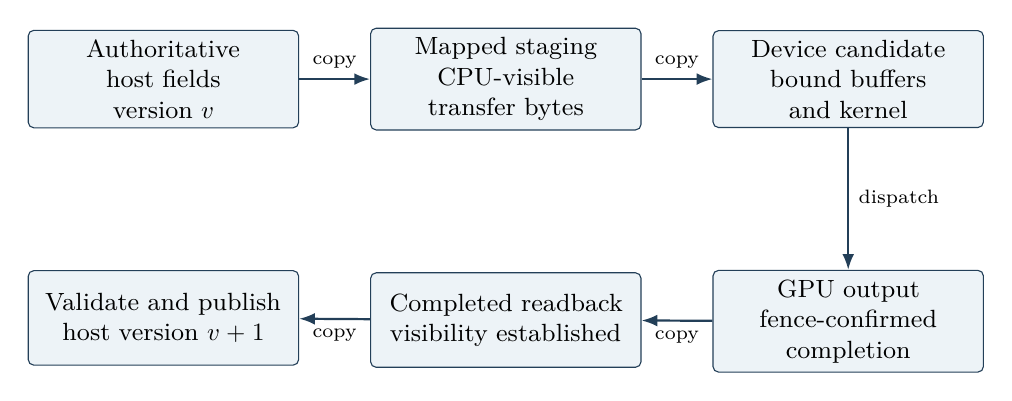
\begin{tikzpicture}[
  box/.style={draw=NimbusBlue,fill=NimbusLight,rounded corners=2pt,
              text width=3.2cm,minimum height=12mm,align=center,font=\small},
  arrow/.style={-{Latex[length=2mm]},draw=NimbusBlue,thick},
  node distance=18mm and 9mm]
  \node[box] (host) {Authoritative host fields\\version $v$};
  \node[box,right=of host] (staging) {Mapped staging\\CPU-visible transfer bytes};
  \node[box,right=of staging] (device) {Device candidate\\bound buffers and kernel};
  \node[box,below=of host] (commit) {Validate and publish\\host version $v+1$};
  \node[box,below=of staging] (readback) {Completed readback\\visibility established};
  \node[box,below=of device] (done) {GPU output\\fence-confirmed completion};
  \draw[arrow] (host)--node[above,font=\scriptsize]{copy}(staging);
  \draw[arrow] (staging)--node[above,font=\scriptsize]{copy}(device);
  \draw[arrow] (device)--node[right,font=\scriptsize]{dispatch}(done);
  \draw[arrow] (done)--node[below,font=\scriptsize]{copy}(readback);
  \draw[arrow] (readback)--node[below,font=\scriptsize]{copy}(commit);
\end{tikzpicture}
\caption{A representative staged-memory compute transaction. Direct shared
memory can remove the separate staging transfer, but still requires ordered
access and an authoritative version transition. The placement of validation
and commit is an operator contract; uncertain GPU execution cannot release
the resources it may still reference.}
\label{fig:architecture-staged-memory}
\end{figure}


\subsection{An uncertain submission cannot release its buffers}

The current compute owner records and submits one shared command buffer at a
time. A successful queue submission means the queue accepted work, not that
its outputs are ready. Completed-operation counters advance after fence
confirmation and required visibility handling. Kernel counts are associated
with that completed submission, so a failed or abandoned command is not
reported as successful native science.

If submission or waiting leaves execution uncertain, the backend is poisoned
and referenced resources remain pinned until shutdown. Reusing a pool slot
after a timeout could let the GPU write into a later unrelated operation.
The pure \href{../vulkan/include/compute/vulkan_submission_lifecycle.hpp}{submission
lifecycle} models this independently of real handles so fault tests can cover
the decision. A host fallback is possible only where the enclosing runtime
allows it and retains a separate valid host state; native-required admission
does not become optional because a device failed.

\section{Residency is a versioned authority graph}

A field allocation can exist without containing the current field. Nimbus's
\href{../include/compute/compute_residency.hpp}{residency graph} records a
logical version, host version and device version together with host identity
and extent. A host write advances the logical version and host version; a
device write advances the logical version and device version. Synchronization
copies a known version to the other side. Reuse is valid only when the side's
version equals the authoritative version and identity/extent still match.

For example, suppose both copies hold version 7. A host boundary update makes
the host version 8 while the device remains at 7. A subsequent kernel cannot
skip upload merely because its input pointer and allocation handle are
unchanged. Conversely, after a device-only update produces version 9, a host
diagnostic must not read version 8 just because the host pointer remains valid.
The state machine exposes these mismatches; it does not itself execute a fence
or inspect the pointed-to bytes.

\href{../include/compute/resident_field_store.hpp}{ResidentFieldStore}
combines that authority graph with named allocation claims. Replacing allocator
callbacks while claims are live is rejected. Batch acquisition publishes no
partial set if a candidate allocation fails, and the callbacks must outlive
the claims that use them. The store is not thread-safe: the backend must
serialize its transitions. Its destructor intentionally does not call an
allocator that may already have been destroyed; owners needing individual
release use the explicit clear path while the allocator is alive.

Generation identity is especially important for restart, grid movement,
resizing and nested contexts. Pointer reuse by a host allocator is not proof
that an old device value still represents the same simulation field. The
\href{../tests/compute/test_residency.cpp}{residency tests} cover state and
allocation behavior, while full runtime tests must additionally prove that
every actual writer announces its transition. A correct cache state machine
cannot compensate for a producer that silently mutates storage behind it.

\section{Metal follows the same ownership questions with different APIs}

Metal exposes a device, command queue, buffers, pipeline states and command
encoders rather than Vulkan's object model. Nimbus stores their session
identity in
\href{../metal/src/compute/internal/metal_device_context.hpp}{MetalDeviceContext}.
Its synchronous finish path commits the command buffer, waits for completion,
checks the final status and only then advances completion telemetry. GPU start
and end timestamps describe the completed command; host submit/wait time is
a different interval.

Shared-storage buffers make memory CPU- and GPU-accessible on the applicable
device, but a host vector and a Metal buffer created with
\texttt{newBufferWithBytes} are still different owned objects. Creating that
buffer copies bytes. Copying its contents into a solver field after completion
is also real work. Some operators retain resident named resources; others
still allocate or copy through their ordinary paths. A blanket statement that
Metal avoids all transfers would obscure the actual implementation.

Apple's \href{https://developer.apple.com/documentation/metal/choosing-a-resource-storage-mode-for-apple-gpus}{storage-mode guide}
distinguishes CPU-visible shared resources from GPU-private resources. A
private resource may require explicit transfer access when a CPU needs its
data, while shared access still needs correct execution ordering. A private
storage experiment does not become the production policy merely because a
local benchmark can create such resources. Nimbus's
\href{../metal/src/compute/backend/advection.inc}{advection owner} and
\href{../metal/src/compute/internal/metal_resident_state.hpp}{resident state}
show concrete copy and reuse paths.

The backend also checks kernel coverage against the canonical manifest. A
kernel demanding native Float64 arithmetic is reported as hardware-limited
in the current Metal coverage contract; it is not secretly replaced by a
Float32 kernel and called equivalent. Other scientific kernels use explicitly
maintained compensated Float32 formulations. Availability of one family says
nothing about an unrelated family's numerical requirements.

\section{Sharding a simulation across multiple GPUs}
\label{architecture-multigpu}

This section is a design analysis of work Nimbus would need. It does not
describe an implemented distributed solver. The current backend configuration
selects one device index for a compute runtime. The
\href{../vulkan/include/compute/vulkan_device_context.hpp}{Vulkan context}
owns one selected physical device, logical device and compute queue; the
\href{../metal/src/compute/internal/metal_device_context.hpp}{Metal context}
owns one device session and command queue. There is no maintained MPI domain
decomposition or complete multi-device timestep owner in the ordinary runtime.
Multiple runtimes, nested domains, CUDA-assisted kernels and remote SSH
execution do not, individually or together, establish that capability.

\subsection{What is being divided?}

There are three substantially different designs. Independent simulations can
run on different devices without exchanging atmospheric state. Spatial
decomposition instead divides one atmosphere into owned subdomains, which
must exchange the state needed by neighboring numerical operators. Assigning
different physics packages to different GPUs is a third design: for example,
dynamics on one device and radiation on another. That arrangement must move
inputs and return tendencies at their declared cadence. It may duplicate much
of the state and adds a coupling dependency, so it should not be assumed to
solve a memory-capacity problem.

For an initial spatial implementation, horizontal tiles with complete vertical
columns are a reasonable candidate. They keep column radiation, boundary-layer
solves, vertical sedimentation and a column-local implicit solve on one owner.
This is a proposed starting restriction, not proof of support for every current
column formulation. It can produce poor aspect ratios or leave too few tiles
for a large machine. Splitting vertically later would require explicit
distributed column algorithms or gather/scatter phases, including their
memory and synchronization costs. Terrain and moving nests make ownership
more complex even when columns remain whole.

\begin{figure}[htbp]
\centering
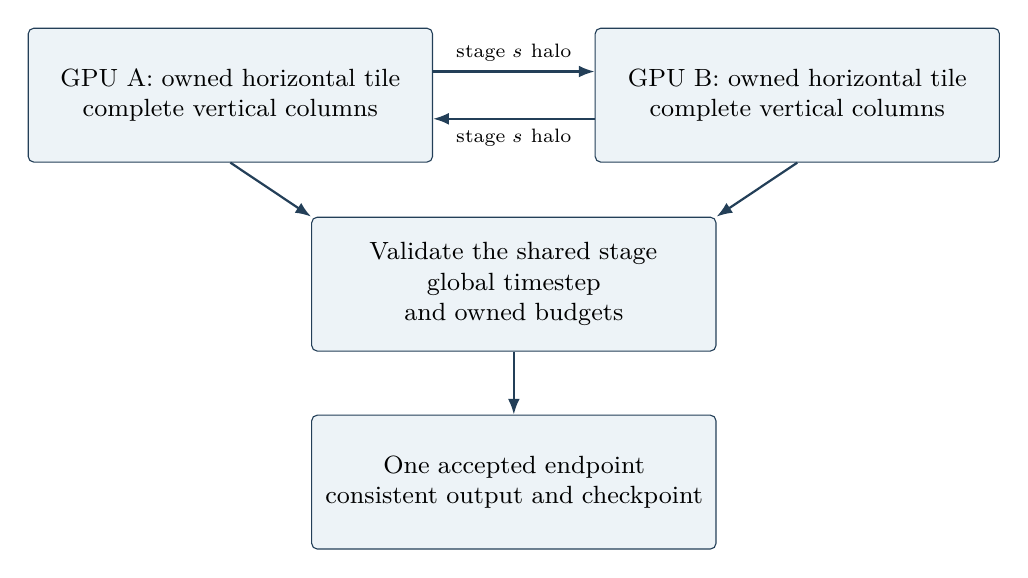
\begin{tikzpicture}[
  box/.style={draw=NimbusBlue,fill=NimbusLight,rounded corners=2pt,
    text width=4.9cm,minimum height=17mm,align=center,font=\small},
  arrow/.style={-{Latex[length=2mm]},draw=NimbusBlue,thick}]
  \node[box] (a) at (0,0) {GPU A: owned horizontal tile\\complete vertical columns};
  \node[box] (b) at (7.2,0) {GPU B: owned horizontal tile\\complete vertical columns};
  \draw[arrow] ([yshift=3mm]a.east)--node[above,font=\scriptsize]{stage $s$ halo}([yshift=3mm]b.west);
  \draw[arrow] ([yshift=-3mm]b.west)--node[below,font=\scriptsize]{stage $s$ halo}([yshift=-3mm]a.east);
  \node[box] (stage) at (3.6,-2.4) {Validate the shared stage\\global timestep and owned budgets};
  \draw[arrow] (a.south)--(stage.north west);
  \draw[arrow] (b.south)--(stage.north east);
  \node[box,below=8mm of stage] (commit) {One accepted endpoint\\consistent output and checkpoint};
  \draw[arrow] (stage)--(commit);
\end{tikzpicture}
\caption{Proposed two-tile solver decomposition. Halo exchange can use a
validated direct path or explicit host staging. Arrows describe data
dependencies, not a mandatory global barrier after every local operator.
Each tile owns its physical cells once; copied halos carry no additional
atmospheric inventory. This is a design diagram, not a current Nimbus feature.}
\label{fig:architecture-multigpu}
\end{figure}


\subsection{Own physical cells and faces before assigning buffers}

Each tile needs global physical bounds, local storage bounds, halo widths,
neighbors and a stable mapping from global to local indices. A halo is a
readable copy of another tile's state, not additional atmospheric volume.
Inventory reductions must count owned cells once. On a C-grid, a velocity or
mass-flux face shared by two tiles also needs a canonical owner or an equivalent
reconciliation rule. Independently evaluating slightly different fluxes on
both sides can create an interface source even when each local kernel passes
its own conservation test.

For one mass flux $\Phi_f$ oriented from tile $A$ to tile $B$, conservative
exchange requires
\[
 \Delta M_A=-\Delta t\,\Phi_f,\qquad
 \Delta M_B=+\Delta t\,\Phi_f.
\]
The same face, time interval, stage weight and transported carrier must be used
on both sides. Water mixing ratios, number per dry mass and number per volume
cannot share an unspecified scalar convention. Geometry, metric coefficients,
held forcing and scheme-private fields require exchange wherever their
consumers need them. A fixed list of visible plot fields is not a sufficient
halo protocol.

Messages should identify the grid or hierarchy generation, physical interval,
integrator stage, field and location, source and destination ownership, extent
and precision. A completed transfer with the wrong stage is stale data. Halo
width must follow the largest actual dependency footprint of the selected
operator, including reconstruction and corner dependencies; it cannot be
guessed from the nearest-neighbor appearance of the final divergence.

Physical boundary conditions apply at the atmosphere's external boundary.
An internal partition face must not become a wall, sponge or independent open
boundary. Periodic neighbors must close the global topology. A processor
partition on a fixed grid is also different from a coarse/fine nest: the
latter needs metric-aware restriction, prolongation and flux reconciliation,
not merely a copy between equal-resolution halos.

\subsection{Exchange at the stage that consumes the data}

A portable first implementation could establish this sequence for each
operation with neighbor dependencies: complete the producing work, pack the
required owned boundary state, start its transfers, compute independent
interior cells, complete and unpack the receives, then compute the boundary
region. The new endpoint becomes visible only after all required regions
and validations complete. Packing, transfer and unpacking each retain buffer
ownership until their respective completion events.

This sequence must be derived from the actual split integrator. Acoustic
substeps may require pressure and face-wind exchange several times during one
slow step. Runge--Kutta stages consume their own stage state. Exchanging only
after a complete outer timestep is generally insufficient. A global CFL
decision must use the most restrictive participating tile; a local reduction
does not establish the safety of the global timestep. Iterative diagnostics
or solvers can add global reductions beyond those required by local stencils.

The current \href{../include/compute/dispatch_graph.hpp}{dispatch graph}
describes field hazards, but is not a distributed execution engine. It would
need region and device ownership, explicit exchange edges and completion
dependencies. Likewise, the
\href{../include/compute/compute_residency.hpp}{residency contract} would need
to distinguish an owned interior version from a halo version for a particular
stage. Marking an entire array ``current on the device'' cannot express that
one boundary slab has not arrived.

\subsection{Portable communication first, optional direct paths second}

The reference transport should work with explicit device-to-host transfer,
owned host send/receive buffers and host-to-device transfer. This gives a
testable route without assuming peer access. On a single machine the exchange
can be managed within one process or across explicitly owned processes.
Across machines, MPI is a plausible transport and collective layer. Its
\href{https://www.mpi-forum.org/docs/mpi-4.1/mpi41-report/node235.htm}{nonblocking
neighborhood operations} provide an interface for neighbor exchange, but
posting a nonblocking operation is not proof of overlap or completion. Progress,
thread support and the application's wait schedule must be measured and
validated. The transport does not know Nimbus's field units or stage semantics.

Direct device transfers are optional optimizations of the same exchange
contract. Vulkan device groups are enumerated compatibility groups; they do
not promise that arbitrary installed GPUs can be treated as one memory pool.
The \href{https://docs.vulkan.org/guide/latest/extensions/device_groups.html}{Khronos
device-group guide} and
\href{https://docs.vulkan.org/refpages/latest/refpages/source/vkGetDeviceGroupPeerMemoryFeatures.html}{peer-memory
query} describe the relevant capability checks. Separate logical devices
instead require a supported sharing/transfer mechanism with explicit lifetime
and synchronization rules. A queue barrier or fence on one independent device
does not by itself establish that another device can consume the bytes.

Metal similarly requires using the devices actually exposed by the system.
Apple documents
\href{https://developer.apple.com/documentation/metal/multi-gpu-systems}{multi-GPU
systems} and
\href{https://developer.apple.com/documentation/metal/transferring-data-between-connected-gpus}{transfers
between connected GPUs}. Availability depends on hardware and API support;
multiple packages or dies inside a product do not imply multiple independently
selectable Metal devices. Unified CPU/GPU memory on one device does not establish
peer access to another computer or accelerator.

``GPU-aware MPI'' also needs a specific memory API, transport and build. For
example, \href{https://docs.open-mpi.org/en/v5.0.8/tuning-apps/networking/cuda.html}{Open
MPI's CUDA support} describes supported CUDA-buffer paths. It does not certify
arbitrary Vulkan allocations or Metal buffers. Nimbus would need a validated
interoperability path or host staging for those owners. An unavailable direct
path may select an explicitly supported staged transport; it must not silently
change the numerical operation or violate a native-execution requirement.

\subsection{Why more memory does not imply linear speedup}

Let an illustrative cubic owned tile have side $n$, halo depth $h$, $F$
communicated scalar-equivalents and $b$ bytes per scalar. Its owned payload is
$bFn^3$. A complete surrounding halo occupies
\[
 B_{\mathrm{halo}}=bF\big[(n+2h)^3-n^3\big]
 =bF(6hn^2+12h^2n+8h^3).
\]
If only the six face slabs are communicated in an exchange, their leading
payload is $6bFhn^2$; corners, staged directional exchanges and non-scalar
locations change the exact count. This is a teaching model for an interior
tile, not the traffic of a particular Nimbus kernel. As a fixed global problem
is divided into more pieces, the surface-to-volume ratio grows. Full-column
horizontal tiles have a different geometric count but the same concern.

For message startup cost $\alpha$, effective transfer bandwidth $\beta$,
$m$ messages and payload $B$, a simple model is
\[
 T_{\mathrm{exchange}}\simeq m\alpha+B/\beta
       +T_{\mathrm{pack}}+T_{\mathrm{unpack}}.
\]
With perfect interior/exchange overlap, and with boundary work and a collective
following those phases, a stage still takes roughly
\[
 T_{\mathrm{stage}}\gtrsim
 \max(T_{\mathrm{interior}},T_{\mathrm{exchange}})
 +T_{\mathrm{boundary}}+T_{\mathrm{collective}}.
\]
Real overlap can be worse: packing can contend for memory bandwidth, transfer
engines may share links, and small tiles can underfill a GPU. Frequent acoustic
exchanges can become latency-bound. A second board behind a narrow or shared
link may increase capacity while adding little useful throughput.

Every device must fit its own owned state, halos, stages, rollback and
communication buffers. The sum of nominal VRAM capacities is not an admission
test. Nor should every rank retain a full global host mirror: that would
preserve a memory bottleneck even after the device fields were partitioned.
NUMA placement should associate host staging buffers and communication threads
with the relevant device and network path. On heterogeneous GPUs, equal cell
counts need not give equal stage times. Cloud-dependent work and nested
placement can also make the slowest tile change during an experiment.
Dynamic balancing would require a state migration transaction and new
generations, not just moving an array pointer.

\subsection{Global diagnostics, restart and failure must agree}

Budget reductions should accumulate owned physical inventories with declared
precision and ordering. A reduction tree may change rounding when the number
of ranks changes. Fixed-decomposition repeatability, decomposition-independent
bitwise equality and bounded scientific agreement are distinct claims. They
need distinct tests; ordinary parallel summation does not promise all three.
Random perturbations should have a defined mapping to physical identities and
time if results are intended to be independent of rank placement.

A checkpoint needs a globally consistent accepted endpoint: all owned primary
and private fields, geometry, held-source clocks, histories, configuration and
publication identity. Repartitioned restart needs a mapping from saved physical
ownership to the new layout; it cannot depend on finding the same GPU index.
Partitioned output should publish a manifest only after all required pieces
are durable, and readers should reconstruct the logical field without treating
rank order as a coordinate system. Gathering the whole atmosphere on one rank
for every frame can become a new memory and I/O bottleneck. Existing NPY,
netCDF and ZFP support does not by itself supply this distributed publication
protocol, and this design does not authorize removal of NPY.

If one tile rejects a timestep, neighboring tiles cannot publish a mixture of
old and new endpoints. A first design should stop the distributed job on an
unrecoverable device or communication failure and resume from a validated
global checkpoint. Transparent continuation after losing a rank is additional
engineering, not a consequence of using MPI. Buffers involved in uncertain
device submissions must remain owned until completion is known or the
corresponding execution context has been safely retired.

\subsection{A sequence that can be implemented and reviewed}

Begin with the distributed state and exchange contract, including a one-tile
path that reproduces the existing admitted experiment. A two-tile CPU or
host-staged reference can then expose ownership errors independently of peer
transport. Manufactured fields should cross each partition orientation and
corner; interface inventories must cancel, and halos must never enter physical
budgets. Tests should mutate stage identities, interrupt transfers and reject
partial publication.

The next bounded target is a two-device, fixed-grid configuration with stated
physics and boundary conditions, selected through ordinary public configuration.
It needs whole-step one-device comparisons, native dispatch evidence, restart
on the same decomposition, rejected-input atomicity and memory accounting.
Changing the decomposition on restart, nonuniform hardware, terrain, private
microphysics state, held radiation, nesting and moving domains each extend the
contract and require their own completed coupling. They cannot be called
supported merely because the flat dry exchange works.

Only after correctness should direct peer transfers, overlap, larger device
counts and multi-node transports be assessed with strong- and weak-scaling
experiments. Strong scaling holds the physical numerical problem fixed; weak
scaling holds approximately the work per participant fixed and generally grows
the global problem. Report both completion time and resource cost, including
output and restart. Source code or a two-GPU speedup alone is not Ready, and
Ready remains separate from campaign validation and independent scientific
review. This staged design keeps the ordinary local workflow usable while
making distributed execution an explicit, testable extension.


\section{Floating-point semantics across CPU and GPU}
\label{architecture-numeric-portability}

\subsection{Storage precision, arithmetic precision and rounding points}

Binary32 has 24 bits of significand precision, including its implicit leading
bit for normal values; binary64 has 53. Their unit roundoffs near one are
approximately $2^{-24}$ and $2^{-53}$ under round-to-nearest. Storing the main
fields as Float32 therefore limits what a wider intermediate can publish.
If a source computes a tiny increment in double precision and then stores
\texttt{float(old + increment)}, that increment can disappear at the storage
boundary. It is not necessarily safe to move the cast earlier, because an
intermediate rounding can also change a threshold decision or cancellation.

Nimbus's dry EOS deliberately evaluates from stored Float32 density and theta
using wider arithmetic before storing pressure. Energy attribution distinguishes
ideal changes from water, theta and pressure storage effects. Backend work must
preserve the intended rounding points and constants. A tolerance patch that
makes one Linux failure disappear without explaining the changed operation
would conceal a numerical portability problem rather than solve it.

\subsection{FMA is useful precisely because it changes rounding}

A fused multiply-add evaluates $ab+c$ with one final rounding, whereas separate
operations compute a rounded product before the sum. Schematically,
\[
 \operatorname{fma}(a,b,c)=\operatorname{RN}(ab+c),\qquad
 \operatorname{RN}(\operatorname{RN}(ab)+c)
 \text{ need not be equal.}
\]
The distinction is especially visible when $ab$ and $c$ nearly cancel.
Compensated algorithms can intentionally use FMA to recover a product residual:
if $p=\operatorname{RN}(ab)$, then $e=\operatorname{fma}(a,b,-p)$ captures the
remaining portion under the algorithm's finite-range assumptions. Reassociating
that expression or replacing it with an ordinary multiply and subtract defeats
the construction.

Even a helper named \texttt{fma\_vectors} needs its concrete implementation
examined. Nimbus uses the fused AVX intrinsic when \texttt{\_\_FMA\_\_} is
compiled, separate multiply/add in the SSE and non-FMA AVX branches, and a
Neon fused intrinsic in its AArch64 vector branch. Scalar tails have their
own compiler contraction behavior. Thus a name alone does not establish
bitwise-identical evaluation on every architecture. Scientific kernels with
stronger requirements use their own explicit arithmetic contracts.

\subsection{Compensated pairs and device capability gates}

Several GPU kernels represent a more accurate intermediate as a high/low
Float32 pair. Addition and multiplication propagate low-order residuals with
carefully ordered fused operations. This increases useful precision for a
defined calculation, but it is not a universal replacement for IEEE binary64:
the exponent range, subnormal behavior, transcendental functions and final
storage conversion still need their own treatment. The
\href{../metal/include/compute/metal/shaders/terrain/mapped_scalar_math_msl.hpp}{mapped
scalar Metal helper} is generated from shared arithmetic sources rather than
being separately hand-tuned into a different equation.

Vulkan distinguishes ordinary Float32 kernels from those explicitly requiring
Float32 storage with Float64 arithmetic. The latter are gated on the required
Float64 rounding/preservation properties, strict Float64 FMA and integer
storage-conversion capability. Compensated families also require the relevant
Float32 signed-zero/NaN preservation and round-to-nearest controls. A device
advertising basic compute support or a high peak throughput number does not
thereby satisfy these scientific requirements.

Tiny values introduce another issue: devices can flush subnormal arithmetic
to zero. The maintained
\href{../vulkan/shaders/compute/terrain/compensated_storage.glsl}{storage helper}
scales tiny inventories before arithmetic and uses explicit integer-bit
rounding for the subnormal storage case. That is an algorithm-specific
representation technique with tests, not permission to add platform-specific
epsilon clamps to every failed comparison. Metal's retained compile policy
disables fast math for these owned shader sources; generator checks keep
translated arithmetic synchronized.

The practical validation sequence follows the contract: check invalid inputs
and output atomicity, compare the intended operator against its independent
reference, test native and generic CPU builds where applicable, then exercise
the real selected backend and memory policy. Exact saved-state comparison,
bounded numerical tolerance and scientific closure remain distinct evidence.
Neither a portable build nor a parity test alone proves that every tracked
configuration is Ready.


\section{Publication, compression and persistent state}
\label{architecture-publication}

\subsection{A frame is published by a protocol}

The output layer translates a completed model state into selected products.
It resolves the field inventory and units, stages required values, encodes
their storage representation and publishes metadata identifying the completed
frame. The existence of a directory or one field file is not enough to tell
a reader that all required fields belong to one finished step. Studio's frame
discovery uses publication state and manifest identity to avoid displaying a
mixture of old and partially written new data.

\href{../src/core/output/output_writer.cpp}{AsyncOutputWriter} has synchronous
and asynchronous paths. A synchronous writer can use a valid borrowed view
while the caller holds the state stable. A background writer requires owned
snapshot storage; \texttt{submit} rejects a borrowed field rather than letting
the integration thread mutate data while compression reads it. Its queue has
a one-frame ownership bound, and the ordinary runtime waits for availability
before assembling the next full snapshot. Backpressure is deliberate: an
unbounded queue would convert a slow filesystem into uncontrolled RAM growth.

An asynchronous writer does not remove serialization or compression work. It
allows some work to overlap while introducing a snapshot, queue synchronization
and a separate error path. A write failure sets an error state and wakes waiting
participants so that an output error cannot strand the producer indefinitely.
The scientifically relevant frame remains identified by model time and source
state, not by the wall-clock moment when the filesystem completes its write.

NPY provides a direct array format, netCDF provides structured scientific
history, and ZFP provides selected compressed representations. Their wrappers
must preserve axis order, shape, field identity and physical metadata. Internal
storage order need not be the order a downstream VTK image expects; that
conversion belongs to the reader/preparation boundary. A decoder that produces
the right number of floats in the wrong order has not preserved a field.

\subsection{What ZFP contributes, and what Nimbus adds}

Peter Lindstrom's 2014 paper, \emph{Fixed-Rate Compressed Floating-Point Arrays},
develops a block representation intended to make compressed numerical arrays
accessible at a prescribed storage rate. Small $4^d$ blocks in $d$ dimensions
share a floating-point representation, undergo a decorrelating transform and
are encoded by significance. The paper supplies the codec method; it does not
specify Nimbus's history container, keyframe schedule, field tolerances or
publication transaction. See the
\href{https://vis.cs.ucdavis.edu/vis2014papers/TVCG/papers/2674_20tvcg12-lindstrom-2346458.pdf}{primary paper}.

The current library's modes answer different questions. Fixed rate constrains
bits per value/block, while error depends on the data. Fixed precision controls
encoded transform precision; it is not a uniform pointwise relative-error
promise for every value in a mixed-magnitude block. Fixed accuracy targets an
absolute error scale in the field's units and produces variable-length output.
Reversible mode supplies bit-preserving reconstruction. These mode distinctions
are defined by the versioned
\href{https://zfp.readthedocs.io/en/release1.0.1/modes.html}{ZFP 1.0.1 mode reference}.
The library also documents finite-representation limits for exceptionally small
accuracy tolerances. Zero tolerance in a lossy mode must not be described as
equivalent to reversible compression; see
\href{https://zfp.readthedocs.io/en/release1.0.1/faq.html}{FAQ questions 17, 20 and 21}.

Nimbus calls the corresponding stream setters in its output writer and records
the mode parameters in its own container. Ordinary public mode parsing accepts
\texttt{accuracy}, \texttt{precision} and \texttt{rate}; admission imposes
additional restrictions for a supported scientific profile. The retained
ordinary admitted lossy-history contract requires accuracy mode and per-field
tolerances, prohibits a positive sparse threshold and disallows the optional
Float16 prefilter. Configuration code also caps the potential-vorticity
tolerance at $10^{-8}$ in its SI representation: a generic visual tolerance
could erase a meteorologically significant signal while still being a valid
codec setting. These are Nimbus decisions in
\href{../src/core/output/output_config.cpp}{output configuration}, not universal
recommendations from the compression paper.

The optional sparse and Float16 transforms are separate lossy operations before
compression. The former sets eligible small values to zero; the latter rounds
eligible values to reduced significand precision. A codec tolerance applies to
the values supplied to that codec. It does not retroactively bound information
already removed by a prefilter. For a source $x$, prefilter $F$, codec
reconstruction $D(C(F(x)))$ and later reconstruction $R$, a useful accounting
separation is
\[
 |x-\widehat x|
 \leq E_{\mathrm{prefilter}}+E_{\mathrm{codec}}+E_{\mathrm{reconstruction}},
\]
when the individual terms have actually been defined and bounded for that
path. Writing down the inequality does not prove all three bounds. This is why
the admitted policy restricts transforms and why quantitative output checks
must compare the final decoded field, not just inspect a mode name.

Temporal delta history is another wrapper-level choice. The encoder keeps
decoded previous fields so that the reader and writer predict from the same
represented history. For a linear two-frame predictor, the conceptual equations
are
\[
\begin{aligned}
 P_n &= 2\widehat x_{n-1}-\widehat x_{n-2},\\
 r_n &= x_n-P_n,\\
 \widehat x_n &= P_n+\widehat r_n.
\end{aligned}
\]
The implementation computes residual and reconstruction expressions with
specified wider intermediates and Float32 storage. With identical predictor
history, old error is already incorporated in the residual definition; using
uncompressed previous fields at the writer and decoded previous fields at the
reader would introduce a different drift mechanism. Actual error still
includes residual rounding, codec error and final reconstruction rounding.
Keyframes reset history dependencies, and retention cannot remove a frame
that a retained delta chain still needs.

Nimbus's spatial container bricks are also different from ZFP's internal
$4^d$ codec blocks. The current bricked reader can select $64\times64\times32$
container bricks, inspect a directory of offsets and reconstruct only the
required spatial region for supported versions. Legacy containers can require
full-volume reconstruction. A small requested output window therefore does
not always imply a small decode working set. The native reader reports these
capabilities instead of silently labeling a full decode as a cheap window.

Field-parallel publication assigns independent fields to workers with isolated
codec workspaces; libzfp execution within each field remains serial in this
policy. It is not the same as enabling the library's internal parallel codec.
Scratch budgets and exact serial/parallel artifact checks are part of the
wrapper contract. More workers may improve throughput, increase memory
pressure, or do neither; the retained benchmark harness makes no universal
throughput claim. The
\href{../tests/core/test_zfp_roundtrip.cpp}{roundtrip tests} and
\href{../tests/integration/test_zfp_field_parallel_benchmark.py}{benchmark
contract tests} address different parts of this behavior.

The reversible radar-v4 container uses the library's reversible mode and
per-brick integrity information under a separate guarded mixed-history path.
It must not be used to claim that ordinary lossy output is exact, or that the
general radar-v4 readiness work is complete. Output history is also not the
solver's in-memory representation: this architecture does not generally
compress prognostic arrays in place between numerical operators. Paper results
about compressed numerical-array computation cannot be transferred to Nimbus's
history writer without a separate implementation and measurement.

\subsection{Checkpoints encode continuation, not just visible fields}

A restart needs more than wind, temperature and water arrays. It can require
scheme-private particle state, time/cadence counters, boundary history, nested
execution state, trajectories and other runtime owners. The checkpoint layer
serializes a versioned set of sections rather than writing the raw bytes of a
C++ object graph. Raw pointers, allocator state, vtable addresses and mutexes
have no portable meaning in another process.

\href{../include/core/runtime/checkpoint_format.hpp}{The wire format} uses
explicit little-endian integer encodings and IEEE floating-point values,
section identifiers, versions, lengths, flags and checksums. It rejects
duplicate or unsupported required sections and checks sizes before allocation.
The architecture-specific in-memory layout is therefore separated from the
continuation format. A native reader can convert byte order where needed;
compatibility still depends on supported versions and the semantic state
contract, not merely on recognizing the file magic.

The writer streams sections into a temporary file while computing integrity
information, closes and synchronizes it, atomically publishes the destination,
then synchronizes the containing directory through platform helpers. This
avoids treating a partial file as the final checkpoint. On restore, decoded
candidate state and attachments are validated before replacing the live state.
An unknown future section or inconsistent tracking authority must not become
a partially restored simulation. See
\href{../src/core/runtime/simulation_checkpoint.cpp}{checkpoint assembly and restore},
\href{../tests/core/test_checkpoint_wire.cpp}{wire tests} and
\href{../tests/core/test_simulation_checkpoint.cpp}{continuation tests}.

\section{Studio IPC, asynchronous work and remote execution}
\label{architecture-ipc}

\subsection{Keep native resources behind the Rust boundary}

Studio's React components express user intent and maintain view state. Rust
owns native filesystem and process operations. Tauri commands carry typed
requests and responses across that boundary. A field-window response uses a
compact binary envelope with a small validated header and Float32 payload,
rather than inflating millions of values into a JSON number array. Geometry
may add aligned Float64 components when required by the declared schema.

The native command checks source dimensions, range, stride, output count,
arithmetic overflow and byte limits before serving the request. Its current
window limits distinguish 64 MiB of returned field data from a larger bounded
source working set. A shared native I/O reservation budgets source bytes plus
twice the output bytes under a 512 MiB aggregate ceiling, then releases the
claim through RAII when the last owner drops it. This models simultaneous
work, not just the size of an individual successful response. See
\href{../ui/src-tauri/src/commands/outputs.rs}{native field commands} and
\href{../ui/src-tauri/src/commands/io_budget.rs}{I/O reservations}.

These values are implementation ceilings, not a promise that every computer
can safely devote that amount to Studio. Frontend preparation and GPU textures
have additional budgets. A renderer can be within its texture-size limit yet
run out of combined native, JavaScript and GPU working memory. The system must
retain the reason a representation was reduced or refused rather than silently
labeling it full resolution.

\subsection{Cancellation is a state transition, not instantaneous preemption}

Each native window read has a request identity, cancellation flag and phase.
Cooperative loops check the flag during header reading, streaming and other
interruptible work. A libzfp decode or native netCDF hyperslab call cannot be
interrupted at an arbitrary instruction through this interface. Cancellation
is checked at its boundaries; a cancelled result is then discarded. The
receipt says cancellation was requested, not that an in-progress native call
has already stopped.

The frontend has a complementary obligation: a late result from frame $n$ must
not replace frame $n+1$ after the user scrubs forward. Request/generation
identity and coherent scene publication solve a different problem from the
native cancellation flag. Even a request too late to cancel can be prevented
from publishing into the wrong view. The
\href{../ui/src/lib/run/frameIdentity.ts}{frame identity} and
\href{../ui/src/lib/vtk/coherentSceneGeneration.ts}{scene generation}
owners make that distinction explicit.

JavaScript workers perform preparation and extraction outside the main UI
thread. Transferable ArrayBuffers move ownership and detach the transferred
buffer; SharedArrayBuffers share storage when the environment permits them.
Nimbus's handoff protocol distinguishes a transferred render-only result from
a retained scientific source and from a shared immutable dataset. The choice
must preserve retries and cache users. Avoiding a structured-clone copy is
useful, but does not establish that native IPC or GPU texture upload was
zero-copy.

\subsection{Launching and stopping a process}

The \href{../ui/src-tauri/src/commands/runner.rs}{native process runner}
checks the executable and configuration identities before spawning. It
publishes immutable launch provenance and starts separate readers for stdout
and stderr plus a waiter for process completion. This keeps a child blocked
on a full output pipe from appearing to be a stalled numerical solver. The
process exit state is distinct from a complete final frame or a verified
checkpoint; readers must still inspect publication records.

Stopping is also owned. On applicable Unix paths, the runner requests graceful
termination and escalates if the child does not exit within its grace period.
It does not equate closing a plot with killing the simulation, and a failed
process does not become a successful run merely because it emitted several
valid early frames. Filesystem, process and application lifecycle operations
must preserve their separate error states.

Remote execution stages an exact request on a user-configured SSH target,
checks the remote executable's catalog and identities, and launches that
process there. Receiving output has its own inventory, per-file hashes and
completion/cancellation receipt. A cancelled transfer is not a complete local
copy of the remote run. The
\href{../ui/src-tauri/src/commands/remote_compute.rs}{remote compute owner}
and \href{../ui/src-tauri/src/commands/remote_receive.rs}{receive owner}
separate launching from verified retrieval.

This is remote process orchestration, not MPI domain decomposition. The current
architecture does not automatically distribute one atmospheric grid across
multiple networked hosts. SSH availability, remote CPU ISA, installed library
ABI, GPU capabilities and local viewer support remain separate checks. The
workstation being unavailable prevents new measurements there; it does not
justify inferring their results from a successful local ARM build.


\section{GPU execution and the path from a field to a screen
pixel}\label{gpu-execution-and-the-path-from-a-field-to-a-screen-pixel}

Nimbus uses GPUs for two different jobs. The solver's Metal and Vulkan
compute backends advance atmospheric state. Studio and the standalone
Vulkan viewer turn an available state into an image. Changing a
colormap, camera, opacity or rendering resolution does not change the
simulated atmosphere. Conversely, selecting a solver backend does not
select Studio's rendering API or give its webview direct access to the
solver's GPU buffers.

The \hyperref[architecture-multigpu]{multi-GPU design section} describes what
it would take to partition the solver across devices. That future compute
capability is separate from distributing rendering. Multiple graphics or
compute queues are not evidence that a simulation is already sharded.

\begin{figure}[htbp]
\centering
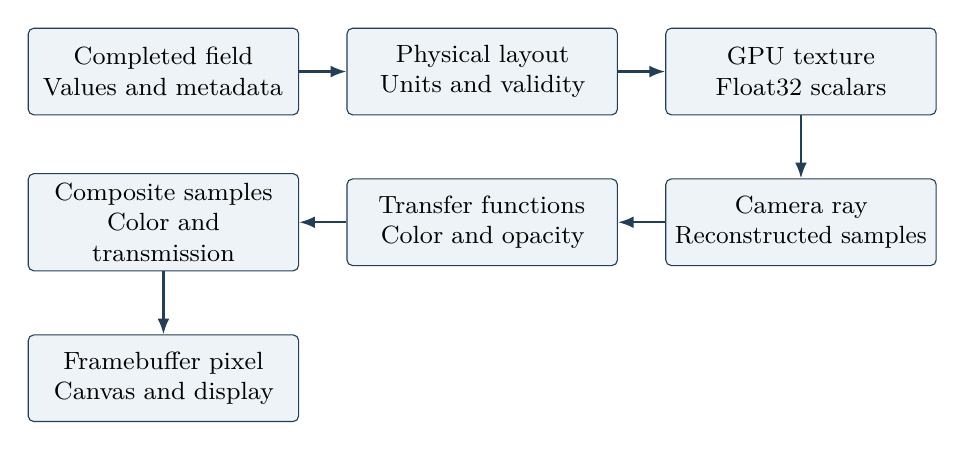
\begin{tikzpicture}[
  box/.style={draw=NimbusBlue,fill=NimbusLight,rounded corners=2pt,
              text width=3.2cm,minimum height=1.1cm,align=center,
              font=\small},
  arrow/.style={-{Latex[length=2mm]},draw=NimbusBlue,thick},
  node distance=8mm and 6mm]
  \node[box] (field) {Completed field\\Values and metadata};
  \node[box,right=of field] (prepare) {Physical layout\\Units and validity};
  \node[box,right=of prepare] (texture) {GPU texture\\Float32 scalars};
  \node[box,below=of texture] (sample) {Camera ray\\Reconstructed samples};
  \node[box,left=of sample] (transfer) {Transfer functions\\Color and opacity};
  \node[box,left=of transfer] (compose) {Composite samples\\Color and transmission};
  \node[box,below=of compose] (screen) {Framebuffer pixel\\Canvas and display};
  \draw[arrow] (field)--(prepare);
  \draw[arrow] (prepare)--(texture);
  \draw[arrow] (texture)--(sample);
  \draw[arrow] (sample)--(transfer);
  \draw[arrow] (transfer)--(compose);
  \draw[arrow] (compose)--(screen);
\end{tikzpicture}
\caption{The volume-rendering path separates scientific values from their
display interpretation. Camera, palette, opacity and lighting affect the image;
they do not advance the atmospheric state. Geometry rendering uses a different
path through vertices, triangles and rasterization.}
\end{figure}


\subsection{Decode the field before interpreting its
appearance}\label{decode-the-field-before-interpreting-its-appearance}

Studio's native Rust layer reads exported NPY, ZFP and netCDF fields,
validates their metadata and returns binary arrays through Tauri. Large
reads can request a bounded spatial window with explicit origin, extent,
stride and aggregation. The window protocol reports the source shape,
returned shape, sample location, missing-data policy and byte
accounting. Its output-byte limit is distinct from the amount of source
data read: computing a block mean still visits the source cells
represented by that block. See the
\href{../ui/src-tauri/src/commands/outputs.rs}{native output reader} and
\href{../ui/src/lib/dataset/nativeFieldWindow.ts}{field-window
protocol}.

The numbers need physical coordinates and units. A dimension named z is
not sufficient evidence of uniform vertical spacing, and closure/halo
storage is not extra atmosphere to display. The reader checks valid
physical ranges, scalar origins, staggering and terrain metadata.
Windowed terrain data can carry double-precision physical centroids and
cell volumes alongside float field values. Studio's Cartesian
preparation resamples stretched or mapped geometry onto the regular
lattice required by a volume image, retaining the interpretation of that
reconstruction.

Units come from the field catalog rather than guesses based on the
variable name. Derived-field recipes declare their inputs and required
units; a saved native field takes precedence over a Studio-derived field
with the same name. For example, temperature derived from theta and
pressure remains a derived diagnostic with a recipe and dependencies. A
horizontal-level anomaly is also a deliberate transformation, not raw
temperature with a different palette.
\href{../ui/src/lib/science/fieldUnits.ts}{Unit labels}, the
\href{../ui/src/lib/derived/derivedFieldRegistry.ts}{derived-field
registry} and \href{../ui/src/lib/science/cartesianInterp.ts}{Cartesian
preparation} own these decisions.

Preparation then repacks values into VTK's x-fastest order. A common
Nimbus array index is \((i n_y+j)n_z+k\); the corresponding VTK scalar
index is \(i+n_x(j+n_yk)\). Setting dimensions without this repack can
silently transpose a non-cubic storm. \texttt{vtkImageData} combines the
scalar array with dimensions, origin and spacing; vectors have three
components per point. Surface geometry instead uses \texttt{vtkPolyData}
with points, connectivity and associated arrays. Neither object is a
framebuffer or an already rendered picture. The
\href{../ui/src/lib/vtk/vtkImageData.ts}{VTK image adapter} is the
central layout boundary; Kitware's
\href{https://kitware.github.io/vtk-js/docs/structures.html}{data-structure
documentation} describes the framework objects.

\subsection{The actual Studio GPU
APIs}\label{the-actual-studio-gpu-apis}

Studio currently selects \textbf{WebGL for volume workloads}, including
when the user prefers WebGPU. Its pinned vtk.js volume path does not
provide the same scene-light, scattering, opacity-normal and
close-camera behavior through WebGPU. This is an explicit workload
policy, not CPU volume rendering. Scientific volume texture code
requires an available WebGL2 context.

Eligible geometry scenes can select WebGPU. Adapter discovery is only
the first check: Studio waits for the mounted
\texttt{vtkWebGPURenderWindow} to initialize its device and confirms the
active API before reporting it active. Missing support, initialization
failure or device loss leads to the documented WebGL compatibility path
and scene reconstruction. The authoritative policy is
\href{../ui/src/lib/vtk/vtkBackend.ts}{vtkBackend.ts}; upstream WebGPU
availability alone does not override it.

A vertex shader transforms mesh vertices into camera/clip coordinates
and passes attributes onward. Rasterization determines the screen
fragments covered by triangles or lines. A fragment shader computes
color and opacity for those fragments. Depth and blending operations
determine how their results enter the framebuffer. A compute shader
instead runs explicit workgroups that read and write buffers or images
without inherently drawing triangles. These are distinct pipeline roles
in the
\href{https://docs.vulkan.org/spec/latest/chapters/pipelines.html}{Vulkan
pipeline specification}.

In Studio, worker-based preparation, marching-cubes extraction and
streamline integration are CPU-side JavaScript work even though their
results are drawn by GPU shaders. The WebGL volume ray marcher runs in a
fragment shader, not a solver compute kernel. WebGPU geometry uses
vtk.js's graphics pipeline with Nimbus's
\href{../ui/src/lib/vtk/vtkWebGpuSurfaceLighting.ts}{surface-lighting
adaptation}.

\subsection{Upload a field, then look up a
color}\label{upload-a-field-then-look-up-a-color}

The VTK volume mapper needs a three-dimensional GPU texture. Nimbus's
\href{../ui/src/lib/vtk/volumeScalarSampling.ts}{scalar texture owner}
explicitly disables half-float storage and uploads Float32 scalar data.
It queries the context's 3D texture limit and float-linear filtering
support. If hardware float-linear filtering is unavailable, a shader
fetches the neighboring texels and performs trilinear interpolation
explicitly. That fallback preserves the scalar precision choice rather
than silently switching to a smaller texture format.

Texture dimensions and logical grid dimensions need not coincide. If one
logical axis is too long but the total cell capacity fits, Nimbus packs
the linear scalar sequence into a legal 3D texture and reconstructs its
logical addresses in GLSL. The upload uses \texttt{texSubImage3D} for
the occupied prefix and restores pixel-unpack state afterward. Capacity
failures are reported; texture packing is not permission to discard
cells. See \href{../ui/src/lib/vtk/volumeTexturePacking.ts}{texture
packing} and
\href{../ui/src/lib/vtk/volumeTextureCapabilities.ts}{capability
checks}.

A color transfer function maps a scalar to RGB. For a range-based
palette, the conceptual coordinate is

\[s=\operatorname{clamp}\!\left(\frac{q-q_{\min}}{q_{\max}-q_{\min}},0,1\right).\]

The palette interpolates between color stops at that coordinate. This
changes the display interpretation, not the source array. Signed fields
can use a diverging palette to distinguish opposite signs. A constant
field needs an explicit degenerate-range policy to avoid division by
zero. Studio's dBZ palette uses physical dBZ anchors, so a specified dBZ
value has the same palette color across runs rather than being stretched
to each frame's extrema.
\href{../ui/src/components/plots/VolumeRender3D.tsx}{VolumeRender3D}
applies these transfer functions and publishes their range for the
legend.

Opacity is a separate transfer function. Two samples can have the same
RGB but different visibility. Increasing opacity can obscure interior
structure; changing the color range can make small variations appear
dramatic. Neither operation increases the information resolved by the
simulation. A scientific figure therefore needs its field, units,
transformation, color range and opacity policy, not just the palette
name.

\subsection{How a volume becomes one
pixel}\label{how-a-volume-becomes-one-pixel}

For each covered screen fragment, the camera defines a ray through the
volume. The shader intersects that ray with the volume's
physical/display bounds and samples along the interior interval. A
texture sample reconstructs a scalar from nearby grid values; transfer
functions turn it into a color and opacity. Sampling between grid points
smooths the displayed reconstruction but does not create new atmospheric
resolution.

Opacity must account for distance. If a transfer-function opacity
\(a_0\) is defined over reference length \(\ell_0\), the corresponding
opacity over a ray segment \(\Delta\ell\) is

\[a=1-(1-a_0)^{\Delta\ell/\ell_0}.\]

This is the constant-extinction Beer--Lambert relationship. Without the
distance correction, taking twice as many samples would make the same
column artificially more opaque. Nimbus also converts display distance
back to physical distance: vertical exaggeration must not thicken a
cloud optically simply by stretching its picture. Geometry
spacing/origin, sample budgets and opacity correction therefore change
together. These are visualization extinction controls, not the
atmospheric RRTMG optical coefficients. See
\href{../ui/src/lib/vtk/vtkPhysicalVolumeOpacity.ts}{physical opacity}
and \href{../ui/src/lib/vtk/volumeOpticalDepth.ts}{optical-distance
handling}.

The front-to-back accumulation for premultiplied color \(\boldsymbol C\)
and opacity \(A\) is

\[\begin{aligned}
\boldsymbol C_{n+1}&=\boldsymbol C_n+(1-A_n)a_n\boldsymbol c_n,\\
A_{n+1}&=A_n+(1-A_n)a_n.
\end{aligned}\]

The remaining transmission weights everything behind the accumulated
samples, including the background. Rays can stop when their interval
ends or their remaining transparency is negligible. Nimbus's coherent
sampling uses a stable pixel-dependent phase and shared sampling bins
across bricks, weighting only each brick's owned segment. Otherwise
arbitrary brick edges can change total opacity or create seams.

When several supported cloud/precipitation layers overlap, the joint
renderer samples their local contributions together and combines optical
depth. Drawing each entire volume as an independent translucent object
can yield incorrect overlap ordering. The current joint owner supports
up to four active scalar textures and owns their transforms, sample
budgets and transfer functions.
\href{../ui/src/lib/vtk/coherentVolumeSampling.ts}{Coherent sampling}
and the \href{../ui/src/lib/vtk/jointVolumeShader.ts}{joint fragment
shader} contain the actual accumulation rules.

Lighting modifies the displayed color using normals and scene lights.
Surface normals come from geometry; lit volumes estimate gradients from
reconstructed scalar or declared opacity information. Nimbus corrects
gradient geometry for anisotropic spacing and uses a fixed world-space
key/fill/rim rig rather than letting an automatic headlight change the
material as the camera moves. Certain structural/cloud views also use
volumetric shadow/scattering controls; generic scalar views can remain
unlit. These are visual cues, not a measured photograph or the solver's
solar-radiation calculation. The
\href{../ui/src/lib/vtk/sceneLighting.ts}{lighting owner} records those
choices.

Opaque geometry contributes depth, which the volume path receives
through its z-buffer pass so integration can respect scene occlusion.
Translucent geometry requires blending and ordering; Nimbus has an
explicit \href{../ui/src/lib/vtk/orderedRenderer.ts}{ordered-renderer
adaptation}. The resulting color/alpha image resides in framebuffer
attachments before the browser or native webview composites the canvas
with controls and legends. Display color handling and final finite-bit
pixels are another representation boundary. A screenshot pixel is not an
invertible measurement of the original scalar after lighting, opacity,
overlap and quantization.

\subsection{Surfaces, contours, vectors and missing
data}\label{surfaces-contours-vectors-and-missing-data}

An isosurface answers a different question: where does a reconstructed
scalar equal a chosen threshold? Marching cubes interpolates crossings
inside cells and creates triangles. The GPU draws those triangles; it
does not integrate every volume sample behind them. Surface color can be
uniform or mapped from an attached scalar. A two-dimensional contour
similarly traces a level set on a plane rather than representing
integrated cloud opacity.

Vector glyphs display sampled direction and magnitude. Streamlines
integrate a vector field at one time and then draw polylines or tubes;
they are not automatically particle trajectories through a changing wind
field. Their seed spacing, integration limits and interpolation
determine what is shown. Studio's separate trajectory owner retains that
distinction.

Missing values are not zeros. A finite substitute may be needed to keep
a volume texture valid, but Studio retains a separate validity mask and
samples it in the shader. The mask also protects normal estimation near
gaps. Marching-cubes cells with missing corners are omitted, and
streamline support prevents a line from bridging an invalid region. The
\href{../ui/src/lib/vtk/volumeValidity.ts}{volume mask},
\href{../ui/src/lib/vtk/finiteImageMarchingCubes.ts}{finite
marching-cubes adapter} and
\href{../ui/src/lib/vtk/finiteImageStreamline.ts}{finite streamline
adapter} implement different representations of the same missing-data
obligation.

Level of detail is likewise explicit. Block means, extrema and point
samples answer different questions; averaging dBZ requires its declared
linear- reflectivity aggregation rather than an ordinary logarithmic
mean. Terrain means use physical-volume information where the protocol
declares it. Bricks, overview levels, temporary screen resolution and
ray step size are distinct quality controls. Preparation carries
resource budgets and source/window provenance, and generation ownership
prevents a stale asynchronous result from replacing a newer field.
Finer-looking interpolation cannot be labeled native resolution after a
coarse source window has been selected.

\subsection{Loading concurrency, cancellation and memory preferences}

Studio separates the count of loading workers from the amount of memory
those workers may hold. A worker limit bounds concurrent field reads and
decoding. The shared native I/O limit accounts for a request's declared source
working set plus twice its output allowance, covering the result and encoding
workspace. The JavaScript scheduler also reserves its estimated read cost.
These are admission bounds rather than measurements of the whole process:
field caches, Python's WebAssembly heap, prepared geometry, browser copies and
GPU allocations retain their own owners and limits.

The automatic native I/O allowance is one thirty-second of detected system RAM,
bounded between 512 MiB and 4 GiB, and further limited by the manual ceiling.
That ceiling is one quarter of RAM, bounded between 64 MiB and 16 GiB. If RAM
is unknown, the default is 512 MiB and the manual ceiling is 2 GiB. A saved
preference can select a smaller or larger allowance within the current
computer's permitted range. These policies use detected capacity, not an ARM
or x86 label; neither policy assumes that GPU memory is unified with RAM.

An individual request larger than the allowance is rejected with its required
size. Ordinary contention instead waits on a native condition variable and
checks cancellation. Reservations live with the worker and its completed
payload until the response is handed back or discarded. Reducing the limit
does not erase memory already owned by an active worker. Those workers finish
or cancel, while later reads wait for capacity. The preference is published to
the frontend only after native configuration succeeds. A delayed status reply
cannot overwrite that newer configuration. Budget-related failed plot reads
retry after a changed allowance is applied, without requiring the user to
leave a volume view.

Prefetch belongs to the selected run, field and spatial window. Frame advance
within that selection can join an existing future-frame read. Replacing or
deselecting the field releases that selection's interest; a shared read is
cancelled when it has no remaining consumers. Failed foreground reads do not
start speculative work. Likewise, an empty isosurface releases its old
geometry rather than merely hiding an actor while retaining its buffers.
These lifetimes matter on both unified-memory and discrete-memory computers.

The first ordinary desktop session without a matching saved profile can measure
loading workers after the interface becomes idle. The measurement generates a
2 MiB float32 NPY file and processes sixteen equal read-and-scan jobs per trial.
Each candidate count receives a warmup and three trials; the median determines
throughput. Candidate counts are powers of two through sixteen, bounded by the
detected core count and including that bound. Studio chooses the smallest count
within five percent of the best median throughput. Cancellation and a twenty
second cooperative deadline bound the work; an operating-system read already
in progress must return before it can stop. Temporary files are removed when
the measurement ends. Explicit worker preferences are preserved.

This is a cached-read and CPU-scan heuristic. It does not measure sustained
storage throughput, netCDF or ZFP decoding, every plot's preparation cost,
solver scaling, or GPU execution. The recommendation is associated with the
CPU identity, core count and RAM reported by the native shell. It can be rerun
after workload changes, and manual controls remain available. A successful
short measurement is not a hardware qualification campaign.

Python array previews similarly separate representation from ownership. A
large heatmap initially point-samples a bounded number of cells; zooming selects
finer samples from the retained complete array. The color range remains tied to
the full finite result, and export uses the original dtype and shape. Coordinate
metadata uses explicit metre, radian, model-level or index units. Unknown
physical geometry does not acquire metre labels through a nominal spacing.

\subsection{The standalone Vulkan
viewer}\label{the-standalone-vulkan-viewer}

The native viewer has a separate path under
\texttt{vulkan/src/rendering}. Its export reader loads and transposes
field data, while a shared-memory input can provide live host-visible
frames. These inputs still pass through the viewer's own normalization
and texture upload; they do not alias a Studio texture or a solver
compute buffer.

Its unipolar normalization uses percentile-clipped ranges. Signed data
uses a centered encoding, with zero at 0.5 and opposite signs on
opposite sides; a sampled cross-frame magnitude estimate is used when
available, with a per-frame fallback. Nonfinite values are counted and
replaced by neutral display values. This differs from Studio's explicit
validity-mask behavior. The normalized intensity is therefore not a
universal physical color scale.
\href{../vulkan/src/data/export_dataset.cpp}{ExportDataset} is the
authority.

The viewer allocates R32 floating-point 3D images, checks required
format and linear-filter support, and uploads each active field. A
persistent two-slot ring holds mapped host-coherent staging buffers. CPU
\texttt{memcpy} fills a free slot; image barriers make it a transfer
destination; \texttt{vkCmdCopyBufferToImage} copies the data; a later
barrier makes it shader-readable. Submission uses
\texttt{vkQueueSubmit}, and slot fences protect reuse while earlier work
is pending. The path remains explicit even on shared-memory hardware.
See
\href{../vulkan/src/rendering/volume_backend.cpp}{volume\_backend.cpp}.

The \href{../vulkan/shaders/rendering/volume.vert}{vertex shader} emits
one oversized fullscreen triangle. The
\href{../vulkan/shaders/rendering/volume.frag}{fragment shader}
constructs camera rays, intersects the physically scaled box, samples
the selected fields and accumulates transmittance. It uses a bounded
ray-step count, anisotropy-aware gradients, display palettes, lighting
and background sky. Optional natural/cinematic texture adds procedural
appearance; it is not simulated small-scale cloud structure. This is a
graphics-fragment ray marcher, not Vulkan hardware ray tracing or
marching-cubes surface extraction.

The window renderer acquires a swapchain image, waits for the necessary
frame ownership, submits drawing and presents it with
\texttt{vkQueuePresentKHR}. It prefers an sRGB surface format when
available. Screenshot capture has a separate image-to-buffer readback
while the application still owns the image, with supported
capture-format checks. Ordinary presentation does not require copying
every pixel back to the CPU.
\href{../vulkan/src/rendering/window_renderer.cpp}{WindowRenderer} owns
this final image-to-display boundary.

\subsection{Memory sharing does not erase ownership or
synchronization}\label{memory-sharing-does-not-erase-ownership-or-synchronization}

Studio's \texttt{SharedArrayBuffer} path can avoid a JavaScript copy
between workers and the main thread. When unavailable, it uses
transferable copies with retained-source and retry rules. It also reuses
immutable prepared datasets across camera changes. These are host
handoff optimizations: ``shared zero copy'' does not mean the browser
directly renders the solver's memory or that texture upload costs
nothing. The \href{../ui/src/lib/vtk/vtkDatasetHandoff.ts}{handoff
owner} records the relevant stages and copies.

On discrete GPUs, host and device memory are separate pools; uploads and
readbacks commonly traverse a bus. Unified memory can expose one
compatible allocation to both processors, but capacity, visibility and
execution ordering still matter. The
\href{https://docs.vulkan.org/guide/latest/memory_allocation.html}{Khronos
memory guide} describes these allocation distinctions. Nimbus's solver
Vulkan backend chooses direct host-visible/device-local buffers only
when its memory plan permits them; the staged path has separate host and
device buffers. It uses buffer copies, barriers, fences and noncoherent
flush/invalidate handling as required. Resident reuse additionally needs
valid field identities and generations; reusing an allocation does not
establish that its contents are current.
\href{../vulkan/src/compute/compute_backend_vulkan.cpp}{The compute
backend} owns these rules independently of the viewer's image-upload
ring.

Metal solver operators use declared buffer ownership, including shared
storage paths. \texttt{newBufferWithBytes} and copying from a buffer's
contents are real copies even on unified memory. Command completion
still precedes consuming a result on the CPU. Host diagnostics or output
may require materializing data that otherwise stays resident. Thus
neither ``Metal'' nor ``unified'' guarantees a copy-free full timestep.
The \href{../metal/src/compute/backend/advection.inc}{Metal advection
owner} shows both ordinary copy paths and resident reuse.

\subsection{Rendering quality and numerical precision are separate
contracts}\label{rendering-quality-and-numerical-precision-are-separate-contracts}

Solver fields are commonly Float32, while selected compute kernels use
compensated pairs, fused operations or explicit storage-rounding
handling to preserve their numerical contracts. The
\href{../metal/include/compute/metal/shaders/terrain/mapped_scalar_math_msl.hpp}{mapped
scalar helper} and
\href{../vulkan/shaders/compute/terrain/compensated_storage.glsl}{Vulkan
storage helper} are examples. These are scientific arithmetic choices,
not image-quality settings. The Metal compiler's retained fast-math
policy also belongs to the compute contract.

Rendering instead has its own precision, interpolation, sampling,
texture and display constraints. A visually smooth cloud is not evidence
of a conservative solver, and pixel differences do not by themselves
prove a physics difference. Maintained tests separately cover
\href{../tests/ui/unit/vtk/test_volume_scalar_sampling.ts}{scalar texture
precision},
\href{../tests/ui/browser/specs/volume-validity.spec.ts}{missing-data
rendering}, \href{../tests/ui/browser/specs/joint-volume.spec.ts}{joint
volume composition},
\href{../tests/ui/browser/specs/volume-colormap.spec.ts}{colormaps} and
\href{../tests/ui/browser/specs/vtk-lifecycle.spec.ts}{scene lifecycle}.
Context/device loss disposes stale resources and rebuilds owned state
before reporting a recovered frame. Capability fallback is visible;
renderer availability is separate from native-only solver admission.
These mechanisms explain behavior and limits, without establishing a
universal performance claim or changing any scientific readiness status.


\section{Performance models and the limits of measured evidence}
\label{architecture-performance}

\subsection{Count work at the boundary that is actually limiting}

The Roofline model relates attainable arithmetic throughput to both compute
capacity and data movement. With operational intensity $I=W/B$, where $W$ is
floating-point work and $B$ is bytes transferred at a specified memory level,
its elementary bound is
\[
 P\leq\min(P_{\max},\beta I),
 \qquad
 t\geq\max\left(\frac{W}{P_{\max}},\frac{B}{\beta}\right).
\]
Here $\beta$ is sustained bandwidth at that same boundary. A memory-bound loop
does not reach twice the performance merely because arithmetic width doubles.
Williams, Waterman and Patterson develop this reasoning in
\href{https://www2.eecs.berkeley.edu/Pubs/TechRpts/2008/EECS-2008-134.pdf}{the
primary Roofline report}. It is a useful bound and diagnostic model, not a
prediction that every Nimbus loop reaches a roof.

For Nimbus, the choice of $B$ matters. Counting bytes requested by source
loads is different from measuring DRAM traffic after cache reuse. Host-to-device
traffic is a different boundary again, and shader access to resident VRAM has
another bandwidth. A CPU loop, a PCIe transfer, a GPU kernel and browser
texture upload should not be placed under one unexplained bandwidth number.
Extra validation or output scans can dominate a complete operation even when
its inner stencil has a favorable arithmetic intensity.

The end-to-end consequence follows by separating an accelerated fraction $f$
of runtime from everything else. If that fraction becomes $s$ times faster,
the idealized whole-program speedup is
\[
 S=\frac{1}{(1-f)+f/s}.
\]
This assumes the remaining work is unchanged and introduces no extra overhead.
If a kernel is 5 percent of total time, even eliminating it entirely saves at
most 5 percent under those assumptions. An actual change may add packing,
allocation, synchronization or validation, so the measured result can be worse.
The implication is to identify the costly owner before choosing an optimization,
not to optimize the largest-looking loop by inspection.

\subsection{Why a local speedup can disappear on another machine}

The cross-architecture investigations have exposed three distinct questions:
how much arithmetic an owner performs, how much data its consumers require,
and when the hardware can execute that work. These questions remain useful
without treating an early measurement on one host as a published benchmark or
an acceptance threshold for a class of computers.

For CPU execution, increasing the worker count can stop helping once a shared
cache, memory interface or synchronization point becomes limiting. SMT workers
share physical resources, and thread placement can change which memory and
cache paths an operator uses. Nimbus therefore exposes explicit worker and
OpenMP placement controls and records the execution context. Its topology
policy is a starting point. It does not encode a particular workstation's
best observed count as a universal x86-64 setting.

Pressure-material reuse addresses a different problem: successive acoustic
operations can need unchanged material coefficients while pressure itself
changes. The current owners retain the immutable information under explicit
state preconditions. That can remove repeated work in the pressure owner, but
the complete step also includes transport, boundaries, microphysics, reports
and synchronization. An owner-level improvement is a hypothesis about overall
performance until the full workload is compared. Similarly, removing an upload
is not sufficient if it adds another synchronization or shifts work to a less
favorable point in the dependency chain.

On a device with separate memory, a staged acoustic command includes upload,
execution, download and host publication. A timer around a transfer side can
include waits for preceding work, driver scheduling and visibility operations;
it is not automatically an isolated measurement of PCIe bandwidth. The staged
implementation keeps those phases explicit so they can be attributed and
compared. It must preserve the same boundary and failure semantics as the
shared-memory path before a transfer reduction is considered equivalent.

Power state, memory clocks, link state and competing work can vary between
runs of an identical binary. A monitor sampled at a different cadence from the
kernel trace cannot establish which individual call experienced a particular
state. Nimbus's measurement workflow therefore keeps uncertainty visible and
requires repeated, matched runs. The public repository does not publish a
personal-device baseline here. Current code documents the implemented reuse,
precision and memory-policy choices; broad ARM64, x86-64, NUMA and discrete-GPU
performance conclusions still require the corresponding measurements.

\subsection{A useful optimization experiment preserves the scientific job}

The candidate and baseline must perform the same work: same configuration,
duration, diagnostic cadence, output selection, memory policy, worker count and
admission requirements. Reducing scientific reports or returning fewer fields
can be a product-mode change, but is not an equivalent implementation speedup.
Likewise, a native-required profile cannot obtain an acceptable timing by
silently substituting a host operation.

Use an isolated owner measurement to locate cost, then evaluate the complete
runtime path with warmup identified and repeated baseline/candidate runs.
Alternating order helps reveal drift; a single before/after pair cannot
separate a small change from varying load or operating state. Nested timers
must state which intervals overlap. An acoustic sub-timer included in the
dynamics timer is not an additional independent contribution to total time.

Correctness evidence accompanies the timing: accepted field bytes or declared
numerical comparisons, checkpoints, relevant conservation ledgers, failures,
threading and applicable backend paths. A source-only count of removed
allocations is a hypothesis until the active runtime and retained dataflow
confirm it. A portable test on one generic x86-64 build demonstrates that
artifact's behavior there; it does not prove broad performance optimality.

\section{Maintaining the ownership and provenance boundaries}

Several inexpensive mistakes can invalidate a technically successful change.
A new source writer can omit a residency transition; a reused scratch array
can leave halos unreadably stale; a serializer can change canonical output
while catalog pins remain old; or a cancellation path can release a reservation
while a noninterruptible native call still owns its memory. These failures are
best understood by asking who owns each resource, which generation its values
describe, what constitutes completion, and which outputs must change together.

Maintained tests mirror those boundaries rather than relying on one aggregate
smoke test. SIMD/alias and hardware-policy tests cover CPU representation and
selection. Memory-plan and residency tests cover allocation and authority.
Native backend tests cover actual dispatch, rejection and completion. Output
and checkpoint tests cover publication and continuation. Studio tests cover
preflight, decoding, geometry, missing data, resource lifetime and pixels.
An analytic rendering fixture can expose an axis swap even when a storm image
looks plausible; a hash mutation can expose a stale contract even when a UI
control still renders successfully.

Generated files require their generator's exact contract. Formatting a
generated shader string header or an exact-scope header can break its text
verification without changing the apparent equation. Formatting a source file
whose raw hash is sealed changes that source identity even if serialized output
is unchanged. Such work should be isolated, regenerated and revalidated rather
than mixed into an unrelated scientific or repository cleanup. Archived
evidence must retain the identities it actually tested.

The repository's status vocabulary remains Engineering incomplete, Ready,
Campaign validated, Externally reviewed and Fully qualified. Source inspection,
bounded tests and this technical manual do not collapse those stages. In
particular, complete bookkeeping of an energy change is not proof that the
physical source is correct; a reproducible image is not proof of a physically
validated storm; and a successful one-host benchmark is not a general hardware
qualification.

\section{Primary references and how they are used}
\label{architecture-references}

The references below describe methods and platform semantics. Nimbus's actual
mode choices, ABI, implementation limits and admission remain defined by the
linked maintained source and tests. A paper's results are not measurements of
the current Nimbus executable.

\begin{description}
\item[Compression method.]
Peter Lindstrom (2014), \emph{Fixed-Rate Compressed Floating-Point Arrays},
IEEE Transactions on Visualization and Computer Graphics, 20(12), 2674--2683.
\href{https://doi.org/10.1109/TVCG.2014.2346458}{DOI: 10.1109/TVCG.2014.2346458}.
\href{https://vis.cs.ucdavis.edu/vis2014papers/TVCG/papers/2674_20tvcg12-lindstrom-2346458.pdf}{Primary paper PDF}.
Used for the block-compression design; Nimbus's containers and temporal
predictor are separately specified in the output writer.

\item[Compression modes and limits.]
ZFP 1.0.1 official documentation,
\href{https://zfp.readthedocs.io/en/release1.0.1/modes.html}{Compression Modes}
and \href{https://zfp.readthedocs.io/en/release1.0.1/faq.html}{FAQ}.
Used to distinguish fixed rate, precision, accuracy and reversible operation,
including finite-representation and pointwise-error caveats.

\item[Performance model.]
Samuel Williams, Andrew Waterman and David Patterson,
\emph{Roofline: An Insightful Visual Performance Model for Floating-Point
Programs and Multicore Architectures}, University of California, Berkeley
Technical Report UCB/EECS-2008-134 (2008).
\href{https://www2.eecs.berkeley.edu/Pubs/TechRpts/2008/EECS-2008-134.pdf}{Primary report PDF}.
Used as an operational-intensity bound, not as a fitted Nimbus performance curve.

\item[CPU instruction sets and compilation.]
Arm, \href{https://developer.arm.com/documentation/101028/0009/Advanced-SIMD--Neon--intrinsics}{Arm C Language Extensions: Advanced SIMD intrinsics};
Intel, \href{https://www.intel.com/content/www/us/en/developer/articles/technical/intel-sdm.html}{Intel 64 and IA-32 Architectures Software Developer Manuals};
GCC, \href{https://gcc.gnu.org/onlinedocs/gcc/x86-Options.html}{x86 Options}
and \href{https://gcc.gnu.org/onlinedocs/gcc/x86-Built-in-Functions.html}{x86 Built-in Functions}.
These define architectural and compiler semantics; emitted instructions and
Nimbus's compiled helper branches determine what a particular build uses.

\item[Thread placement.]
OpenMP Architecture Review Board.\par
\href{https://www.openmp.org/spec-html/5.1/openmpse62.html}{OMP\_PLACES}
and \href{https://www.openmp.org/spec-html/5.0/openmpse52.html}{OMP\_PROC\_BIND}.
Used to distinguish worker count, places and affinity. Runtime support and
observed placement remain necessary when interpreting a measurement.

\item[Vulkan ownership and execution.]
Khronos Group, \href{https://docs.vulkan.org/guide/latest/memory_allocation.html}{Memory Allocation},
\href{https://docs.vulkan.org/guide/latest/synchronization_examples.html}{Synchronization Examples},
and \href{https://docs.vulkan.org/spec/latest/chapters/pipelines.html}{Vulkan Pipelines}.
Used for the distinction between allocation types, memory visibility,
completion and graphics versus compute work.

\item[Metal resources.]
Apple, \href{https://developer.apple.com/documentation/metal/choosing-a-resource-storage-mode-for-apple-gpus}{Choosing a resource storage mode for Apple GPUs}.
Used for shared/private resource semantics. The current Nimbus backend's
resource and completion choices are documented separately above.

\item[Rendering framework.]
Kitware, \href{https://kitware.github.io/vtk-js/docs/structures.html}{VTK.js data structures}.
The pinned framework and Nimbus's workload policy, shader adaptations and
permanent rendering tests define actual Studio support.
\end{description}


\section{Repository boundaries}\label{repository-boundaries}

{\def\LTcaptype{none} % do not increment counter
\begin{longtable}[]{@{}
  >{\raggedright\arraybackslash}p{(\linewidth - 2\tabcolsep) * \real{0.5000}}
  >{\raggedright\arraybackslash}p{(\linewidth - 2\tabcolsep) * \real{0.5000}}@{}}
\toprule\noalign{}
\begin{minipage}[b]{\linewidth}\raggedright
Location
\end{minipage} & \begin{minipage}[b]{\linewidth}\raggedright
Maintained responsibility
\end{minipage} \\
\midrule\noalign{}
\endhead
\bottomrule\noalign{}
\endlastfoot
\texttt{include/}, \texttt{src/} & Solver interfaces, state, operators
and orchestration \\
\texttt{vulkan/}, \texttt{metal/} & Native backend code, shaders and
backend checks \\
\texttt{ui/} & Studio frontend and native shell; maintained tests live under
\texttt{tests/ui/} \\
\texttt{configs/} & Public starting configurations \\
\texttt{tests/} & Numerical references, contracts and bounded
fixtures \\
\texttt{scripts/}, \texttt{mk/} & Reproducible build,
validation and operating tools \\
\texttt{docs/} & Current mathematical, architectural and operating
explanations \\
\end{longtable}
}

Build products, downloaded data, simulation output and historical
investigation records are not source dependencies. Generated directories
are ignored by Git. Required runtime tables have explicit provisioning
instructions in \href{BUILDING.md}{the build guide}. A clean
checkout must be able to rebuild and run the maintained checks without
borrowing objects from an old experiment.

\end{document}
